% !TeX root = chap3.tex
% !TeX encoding = UTF-8
% !TeX spellcheck = fr_FR
\documentclass[12pt, a4paper, oneside]{book}
%\usepackage[utf8]{inputenc}
\usepackage{amsmath}
\usepackage{amsfonts}
\usepackage{amssymb}
\usepackage{graphicx}
\usepackage[left=1.5cm, right=5cm, bottom = 1cm, top = 2cm, headheight=16pt,
headsep = 0.5cm, foot = 16pt, footskip = 0.5cm]{geometry}
\setlength{\marginparwidth}{4.5cm}
\usepackage{marginnote}

\usepackage{fontspec}
\setmainfont{Charis SIL}
\usepackage{setspace}
\setstretch{1.1}
\usepackage[french]{babel}
\usepackage[babel=true]{csquotes}

\usepackage{soul}
\usepackage{mdframed}

\usepackage{xargs} % Use more than one optional parameter in a new commands
\usepackage[dvipsnames]{xcolor}


\usepackage{float}
\usepackage{caption}
\captionsetup[figure]{belowskip=-0.5cm}
\captionsetup[lstlisting]{belowskip=-0.25cm}
%\captionsetup[table]{position=above, aboveskip=0pt, belowskip=10pt}
\usepackage{rotating}
\usepackage{rotfloat}

\usepackage{fancyhdr}
\pagestyle{fancy}

\renewcommand{\headrulewidth}{0.5pt}
\renewcommand{\footrulewidth}{0pt}
\fancyhead[L]{Chapitre \thechapter}
\fancyhead[C]{}
\fancyhead[R]{\rightmark}

\usepackage{epigraph}

\newcounter{savefootnote}
\renewcommand{\thempfootnote}{\arabic{footnote}}%

\usepackage{enumitem}

\usepackage[hyperfootnotes=false]{hyperref}
\hypersetup{pdftitle={Robin Cura - Thèse}}
\usepackage[noabbrev, nameinlink]{cleveref}

\usepackage{longtable}
\usepackage{array}

\usepackage{fontawesome}
\usepackage{wrapfig}
\usepackage[style=authoryear-comp,
hyperref,
backend=bibtex,
isbn=false,
doi=true,
url=true,
date=year,
sortcites=false,  % Ne pas changer l'ordre des citations multiples
sorting=nyt % Citations dans biblio : NameYearTitle
]{biblatex}


%%%% Styles chapitres %%%%
\usepackage[Bjornstrup]{fncychap}
\ChTitleVar{\raggedright\LARGE\sffamily\bfseries}


%\usepackage{natbib}

\usepackage[thinlines]{easytable}
\usepackage{makecell}
\usepackage{diagbox}

\renewcommand\theadalign{bc}
\renewcommand\theadfont{\bfseries}
\renewcommand\theadgape{\Gape[4pt]}
\renewcommand\cellgape{\Gape[4pt]}

\usepackage[french, tight]{minitoc}
\dominitoc

\usepackage{listings} % Code
\lstset{
	basicstyle=\ttfamily,
	frame=single
}
%\usepackage{minted}
\renewcommand\lstlistingname{Code}
\renewcommand\lstlistlistingname{Code}
\crefformat{lstlisting}{code~#2#1#3}
\Crefformat{lstlisting}{Code~#2#1#3}

\usepackage[lofdepth,lotdepth]{subfig}
\usepackage{sparklines}

% ------------------------------------- %
% ---------- COMMANDES PERSO ---------- %
% ------------------------------------- %
% ######### TABLES AVEC FIGURES #########
\newcolumntype{M}[1]{>{\centering\arraybackslash}m{#1}}
\newcolumntype{N}{@{}m{0pt}@{}}
\usepackage{tikz}
\usetikzlibrary{calc,shapes,arrows}
\newcommand{\tikzmark}[1]{%
	\tikz[overlay,remember picture] \node (#1) {};}
% ############# SCHEMAS TIKZ ###########
\usepackage{tikz}
\usetikzlibrary{shapes,arrows.meta, shapes.geometric, positioning, patterns}
\usepackage{dashbox}

%%% TABLES
\usepackage{verbatim}
\usepackage{makecell}
\usepackage{multirow}

\usepackage{upgreek}

\setcounter{secnumdepth}{6}
\crefname{paragraph}{paragraphe}{paragraphes}
\Crefname{paragraph}{Paragraphe}{Paragraphes}

\makeatletter
\DeclareRobustCommand{\cnameref}[1]{%
%	\namecref{#1}
	\nameref{#1}%
}%
\DeclareRobustCommand{\Cnameref}[1]{%
	\nameCref{#1} \nameref{#1}%
}

% ###### CREATION D'ENCADRES ###### %

% Encadré pris dans la thèse de Seb Rey
\usepackage[most]{tcolorbox}
\newtcbtheorem[number within=chapter]{encadre}{Encadré}{
	outer arc=0pt,
	arc=0pt,
	breakable,
	enhanced,
	colback=white,
	colframe=black,
	colbacktitle=white,
	titlerule=0pt,
	fonttitle=\normalcolor\itshape}{enc}

\crefformat{tcb@cnt@encadre}{encadré~#2#1#3}
\Crefformat{tcb@cnt@encadre}{Encadré~#2#1#3}

% ###### COMMENTAIRES ###### %


% Surlignement texte (1) + commentaire en marge (2)

\DeclareRobustCommand{\hlorange}[1]{{\sethlcolor{Dandelion}\hl{#1}}}
\DeclareRobustCommand{\hlcyan}[1]{{\sethlcolor{Cyan}\hl{#1}}}

\newcommandx{\toChange}[2]{%
	\colorbox{Dandelion}{#1}\marginnote{\small\hlorange{#2}}%
}

\newcommandx{\Lena}[2]{%
	\colorbox{Cyan}{#1}\marginnote{\small\hlcyan{Lena:\\ #2}}%
}

% Highlight
\newcommandx{\fixref}[1]{\hl{#1}}

% ToDoBox
\newcommandx{\todobox}[2][1=]{%
	~\\	\colorbox{pink}{\parbox{0.9\textwidth}{%
		\vskip5pt
		\leftskip5pt\rightskip5pt
		#2
		\vskip5pt
	}~\\
}
}

% ######### TITRE #########
\usepackage{titling}
\title{Accompagner la modélisation des systèmes de peuplement par l’exploration interactive de données spatio-temporelles}
\author{Robin Cura}
\date{\vspace{-5ex}}
\makeatletter
\newcommand*{\toccontents}{\@starttoc{toc}}
\makeatother




\newskip\bigskipamount   \bigskipamount =20pt plus 4pt minus 4pt
\setlength{\parskip}{0.75em}
\setlength{\parindent}{2em}

\usepackage{titlesec} % Pose problème avec les headers
% Corrigé avec ce code, à mettre pour chaque section
%\let\orisectionmark\sectionmark
%\renewcommand\sectionmark[1]{}%
%\section[Titre TOC]{Titre dans texte}
%\orisectionmark{Titre header}
%\let\sectionmark\orisectionmark

\titlespacing\section{0pt}{16pt plus 4pt minus 2pt}{0pt plus 2pt minus 2pt}
\titlespacing\subsection{0pt}{11pt plus 4pt minus 2pt}{0pt plus 2pt minus 2pt}
\titlespacing\subsubsection{0pt}{11pt plus 4pt minus 2pt}{0pt plus 2pt minus 2pt}
\titlespacing\paragraph{2em}{6pt plus 2pt minus 2pt}{8pt plus 0pt minus 0pt}



% ######### PLAN DETAILLE #########
% Make a TOC without line number when calling \tableofcontents
%\let\Contentsline\contentsline
%\renewcommand\contentsline[3]{\Contentsline{#1}{#2}{}}
\usepackage{pbox}
\usepackage{array}% http://ctan.org/pkg/array



% ###### AVANT-PROPOS CHAP2 ######
\usepackage{multicol}


% ######## Plusieurs ndbp renvoyant à la même ######
\usepackage{footmisc}
% # Et on met un asterisque à la place
\newcommand{\astfootnote}[1]{
	\let\oldthefootnote=\thefootnote
	\setcounter{footnote}{0}
	\renewcommand{\thefootnote}{\fnsymbol{footnote}}
	\hspace*{-.45cm}\footnote{#1}\unskip
	\let\thefootnote=\oldthefootnote
}

% ############ CITATIONS #############
% Citer juste le prénom + nom d'une référence
\newrobustcmd*{\citeauteur}{\AtNextCite{\DeclareNameAlias{labelname}{first-last}}\citeauthor}
% \citeauteur{ref}


\bibliography{Chap3}

\begin{document}
	\setcounter{part}{0}
	\setcounter{chapter}{2}
	\setcounter{secnumdepth}{4}
	%\part{Accompagner la modélisation d'une transformation dans le système de peuplement de l'Europe Médiévale}
		
	\chapter{Paramétrer un modèle dans un contexte de co-construction interdisciplinaire}
	\begin{center}
		{\large Version 2018-04-16}
	\end{center}

	Le modèle, tel qu'il a été présenté dans le chapitre précédent, était un \og état\fg{}, c'est-à-dire que les mécanismes, paramètres et les valeurs de ceux-ci correspondent à une étape d'un modèle amené à évoluer pour répondre aux problèmes soulevés dans la dernière partie (\hl{Ref dernière section chap 2}).
	Dans ce chapitre, nous nous attacherons à présenter le travail de paramétrage réalisé à la suite, ayant abouti à une version plus adaptée aux questions des thématiciens. Le descriptif technique de cette version \og finale\fg{} se trouve dans l'annexe $n$ (\hl{Ref à l'annexe contenant le descriptif technique de la dernière version du modèle.})
	Par paramétrage, nous entendons ici le processus visant à doter le modèle de paramètres (empiriques, \og commensurables\fg{} et techniques (\cref{enc:types-parametres})) lui permettant de mieux répondre aux objectifs fixé en termes de comportements attendus ou d'objectifs quantitatifs. Nous nous attacherons dans un premier temps à expliciter et spécifier ce sens.
	

%		\section{Paramétrer ? Quoi et comment ?}
	
	Avant de préciser le sens du terme \og paramétrage\fg{}, il semble important de définir précisément ce qu'est un paramètre. C'est en particulier nécessaire en ce que ce terme recouvre de nombreux sens selon les champs disciplinaires qui l'emploient, mais aussi, au sein même de ceux-ci, par les différents chercheurs.
	
	\subsection{Différents points de vue sur la définition d'un paramètre}
	
	Au plus général, le nouveau petit Robert définit un paramètre en ces mots :
	\begin{quote}
		\og 1. \textsc{math.} Quantité à fixer librement, maintenue constante, dont dépend une fonction de variables indépendantes, une équation ou une expression mathématique. --- Variable en fonction de laquelle on exprime chacune des variables d'une équation.\\
		2. \textsc{fig.} et \textsc{didact.} Élément important dont la connaissance explicite les caractéristiques essentielles de l'ensemble d'une question.\\
		3. \textsc{par ext.} Élément nécessaire pour juger, évaluer, comprendre (qqch.).\fg{}\\
		\mbox{}~ \hfill \autocite[\textbf{Paramètre}]{robert_nouveau_1993}
	\end{quote}


	Seule la première définition correspond, à grands traits, à ce que l'on attend ici, mais elle est très généraliste, bien que ne correspondant pas pour autant à tous les usages du terme employés dans la littérature.
	
	\subsubsection{En mathématiques, une définition univoque}
	L'acceptation mathématiques d'un paramètre est sans doute celle qui souffre le moins d'ambiguïté : il s'agit des termes fixes d'une équation simple, par opposition aux variables qui en constituent les éléments qui seront amenés à évoluer.
	Par exemple, dans la formulation d'une fonction affine, $f(x) = ax + b$, la valeur de $f(x)$ dépend de la variable $x$ et des paramètres fixés $a$ et $b$.
	Quelles que soient les valeurs empruntées par $x$, ces paramètres demeurent constants. Dans une famille d'équations plus complexes, par exemple le modèle de croissance logistique de population\footnote{
		$\frac{\text{d}y}{\text{d}t} = \alpha y \times (1 - \frac{y}{K})$ d'après \autocite{verhulst1838notice}
	}, l'accroissement de population au cours du temps ($\frac{\text{d}y}{\text{d}t}$) dépend de la valeur de la variable $y$, population à cet instant, ainsi que de deux paramètres, $\alpha$, le taux de croissance, et $K$, la \og capacité d'accueil\fg{}, c'est-à-dire un potentiel maximum de population vers laquelle tend -- et ne peut donc dépasser -- le système modélisé.
	La définition mathématique est donc assez universelle et convient à la quasi-totalité des systèmes d'équations\footnote{A l'exclusion notable des systèmes d'équation paramétriques, où, à l'inverse, le terme de paramètre désigne alors les variables indépendantes.}.
	Il convient toutefois de noter que la différence entre variable et paramètre est une affaire de point de vue, une inversion de perspective menant à échanger les paramètres et variables, tel que décrit dans l'exemple suivant :
	\begin{quote}
		\og For the function $f(x)=ax^2+bx+c$, could we learn something by leaving the expression in terms of the symbols $a$, $b$, and $c$ and seeing how $f(x)$ depends on the parameters? Maybe we could fix $x=2$ and look how $f(2)$ changes as we let $a$ vary.
		
		If we do such manipulations and look at how the output of a function depends on varying a parameter, then we are treating the function as though the parameter were a input variable. But that's OK, as the difference between variables and parameters is really just a matter of perspective.\fg{}\\
		\mbox{}~ \hfill \autocite{nykamp_function_2015}
	\end{quote}
	On peut donc en retenir qu'en mathématiques, ce qui différencie la variable du paramètre est l'aspect fixe de ce dernier, au moins pendant la durée d'exécution d'une fonction : 
	\begin{quote}
	\og{}A parameter is a quantity that influences the output or behavior of a mathematical object but is viewed as being held constant. [\dots]
	Variables are viewed as changing while parameters typically either don't change or change more slowly.\fg{}\\
		\mbox{}~ \hfill \autocite{nykamp_parameter_2015}
	\end{quote}

% Conserver pour experiences etc. \footnote{
%		\og{}In some contexts, one can imagine performing multiple experiments, where the variables are changing through each experiment, but the parameters are held fixed during each experiment and only change between experiments.\fg{}\autocite{nykamp_parameter_2015}

	On propose donc une une définition sans doute plus spécifique que celle du nouveau petit Robert, mais aussi plus tournée vers l'usage : un paramètre est une variable maintenue constante durant l'ensemble de l'utilisation d'une fonction.
	
	\subsubsection{Une vision duale en statistiques}
	En statistiques, quand bien même cette discipline fait un large usage des formalismes mathématiques, les paramètres recouvrent un ensemble assez différent : il s'agit d'une \og grandeur mesurable qui permet de présenter de façon plus simple, plus abrégée les caractéristiques essentielles d'un ensemble statistique.\fg{} \autocite[Paramètre, \textsc{stat.} (calcul des probabilités)]{tresor1992}
	\begin{quote}
		\textit{In statistics}, the most common use of \og parameter\fg{} is for a characteristic of a population, or of a distribution of scores, described by a statistic such as a mean or a standard deviation. For example, the mean (average) score of on the midterm exam in Psychology 201 is a parameter. It describes the population composed of all those who took the exam.\\
		\mbox{}~ \hfill \autocite[164]{vogt1993dictionary}
	\end{quote}
	Ainsi, pour les statisticiens, la moyenne, l'écart-type ou encore le coefficient d'asymétrie sont des paramètres, que l'on symbolise alors au moyen de lettres grecques \autocite[ibid.]{vogt1993dictionary}.
	On peut toutefois y retrouver une logique commune avec les paramètres mathématiques quand on décrit une loi statistique avec ces valeurs, qui deviennent alors les éléments permettant de caractériser une variable. Ainsi, pour décrire les caractéristiques de la distribution théorique -- normale-- d'une variable $X$, on fera appel aux paramètres théoriques de cette loi que sont l'espérance\footnote{Il s'agit de la moyenne théorique. On réserve ainsi le terme de moyenne à une valeur calculée depuis des valeurs empiriques.} ($\mu$) et l'écart-type ($\sigma^{2}$): $X \hookrightarrow  \mathcal{N}(\mu,\,\sigma^{2})$.
	
	\subsubsection{Une absence de consensus en informatique}
	Dans le domaine informatique, la définition est bien plus floue et inclusive que dans les champs décrits auparavant, sans doute en raison d'une hétérogénéité bien supérieure dans les pratiques et construits informatiques. Comme dans les fonctions mathématiques, les paramètres sont les arguments des fonctions informatiques. Ces fonctions recouvrent toutefois un ensemble extrêmement vaste, bien plus hétérogène que dans les domaines mentionnés ci-dessus.
	On parle ainsi de fonction\footnote{On utilisera aussi indistinctement les termes de procédure, de (sub)routine ou encore de méthode. Notons que chacun de ces mots a normalement un sens précis. Par exemple, une méthode désigne une fonction qui peut être exécutée par une instance de classe en programmation orientée objet. Certaines définitions plus précises sont toutefois souvent utilisé à mauvais escient, provoquant alors des inversions de sens. Ainsi, une procédure est le plus souvent décrit comme une suite d'instructions ne retournant pas de valeur, au contraire d'une fonction. Mais, par exemple dans le langage SAS \autocite{sas1990sas}, toute fonction est nommée procédure, à l'instar de la moyenne par exemple (\texttt{PROC MEANS}).} pour toute suite d'instructions informatique ayant pour vocation -- ou pour capacité -- à être répétée, ré-exécutée.
	Ces fonctions appliquent ainsi, le plus fréquemment, cette suite d'instruction sur des données en entrée, et produisent ainsi des données en sortie, résultantes du traitement effectué sur les entrées\footnote{
		Notons que certaines fonctions produisent des \og effets de bord\fg{}, c'est-à-dire ne renvoient pas de données en sortie, mais effectuent une action à partir des données en entrée. La fonction imprimer par exemple, ne renvoie aucune sortie informatique, ce sont ses effets de bord qui déclenchent l'impression d'un document.
	}.
	Certaines fonctions sont donc très simples, et peuvent s'apparenter à des fonctions mathématiques, telles que par exemple la fonction arrondi (\texttt{round()} dans sa version la plus courante). Cette dernière prend en entrée un nombre décimal, et retourne un nombre entier. Le nombre décimal passé en entrée est alors nommé paramètre. Notons que cette fonction accepte le plus souvent un second paramètre, sous forme d'un nombre entier, qui permet de définir le nombre de décimales (\textit{digits}) que l'on souhaite conserver. Par exemple, l'arrondi de $2,551$ à une décimale renverra la valeur $2,6$.
	Il est important de noter qu'en informatique, les paramètres ont souvent une \og valeur par défaut\fg{}, c'est-à-dire une valeur qui sera utilisée si le paramètre n'est pas explicitement spécifié. \change{Lena : vraiment ?}{D'où une confusion fréquente entre paramètre et valeur initiale, en particulier dans le domaine de la simulation à base d'agents.}
	Dans le cas de la fonction arrondi, si le premier paramètre n'a pas de valeur par défaut, ce qui n'aurait aucun sens, le second paramètre est souvent proposé avec une valeur par défaut de $0$. Si on ne la précise pas, le nombre renvoyé par la fonction sera ainsi un entier, soit $3$ dans le cas précédent:
	\texttt{round}$(2.551) = 3$, mais \texttt{round}$(2.551, \text{digits} = 1) = 2,6$.
	
	Ce premier exemple est quasiment en tout point assimilable à l'acceptation mathématique d'une fonction, et dès lors, ses paramètres ressemblent fortement à ceux que ce domaine définit, à l'exception que le premier paramètre de la fonction arrondi serait défini comme une variable en mathématiques. Pour autant, l'informatique fait usage de nombreuses fonctions bien moins comparables, car formulées de manière algorithmique et non mathématique.
	
	Prenons l'exemple d'une fonction simple de conversion d'image, permettant par exemple de convertir une image du format \texttt{JPEG} au format \texttt{PDF}. Cette fonction, que l'on nommera \texttt{convert}\footnote{Cette fonction est disponible dans le logiciel ImageMagick \autocite{imagemagick2008imagemagick}.}, requiert au moins deux \og paramètres\fg{} : l'emplacement informatique (le \og chemin\fg{}, ou \textit{path}) du fichier image (\texttt{JPEG}) d'origine, et le chemin du \texttt{PDF} en sortie. Il ne s'agit plus dès lors de paramètres numériques comme en mathématiques ou en statistiques, mais d'éléments nécessaires à une fonction pour être exécutée.
	De plus, cette fonction accepte aussi d'autres \og paramètres\fg{}, permettant entre autre de redimensionner l'image pendant cette conversion, d'en modifier la résolution, ou encore d'en transformer les couleurs, par exemple en la convertissant en nuances de gris.
	Ces paramètres, facultatifs, agissent alors comme autant de nouvelles fonctions. Ils ne servent plus uniquement à \og paramétrer\fg{} le but premier de la fonction de conversion, mais en fait à y ajouter des fonctionnalités, des mécanismes de transformation de l'image source.
	
	On ne peut donc plus véritablement parler de variables qui seraient affectées ou transformées par des valeurs statiques de paramètres. On utilisera donc, dans ce contexte, davantage le terme de paramètre d'entrée ou encore d'argument dans ce cas. Notons qu'en anglais, la différence entre \textit{parameter} et \textit{argument} est plus formalisée qu'en français : ils se définissent par le lieu de leur utilisation. Lors de la définition d'une fonction, on fait appel à des paramètres qui seront utilisés au sein de la fonction. Lors de l'utilisation de cette fonction, l'utilisateur fournira des arguments, dont les valeurs seront alors utilisés en remplacement des paramètres dans la fonction.
	\begin{quote}
			\og The terms parameter and argument are sometimes used interchangeably, and the context is used to distinguish the meaning. The term parameter (sometimes called formal parameter) is often used to refer to the variable as found in the function definition, while argument (sometimes called actual parameter) refers to the actual input passed. For example, if one defines a function as \texttt{def f(x): ...}, then \texttt{x} is the parameter, while if it [is] called by \texttt{a = ...; f(a)} then \texttt{a} is the argument.\fg{}\\
			\mbox{}~ \hfill \autocite{_parameter_2017} 
	\end{quote}


	\subsubsection*{} Il apparaît donc que si les définitions mathématiques et statistiques d'un paramètre sont assez largement précises et explicites, il en est tout autre dans le champs disciplinaire informatique. Peut-être parce que ce champs est composé de bien plus de praticiens (les développeurs) que de chercheurs, on constate que les termes de variables, de paramètres, d'arguments ou encore d'entrées (\textit{inputs}) y sont assez régulièrement intervertis. Afin de préciser l'emploi que nous ferons de ces termes dans le cadre de la modélisation à base d'agents présentée dans le chapitre précédent, il convient donc de s'intéresser plus spécifiquement aux usages de ces termes dans le domaine de la simulation informatique en sciences humaines.
	
	\subsection{Les paramètres dans les modèles agents}
	
	\subsubsection{L'approche classique}
	
	Un premier point est à noter : nous n'avons trouvé que très peu de définitions spécifiques de ce qu'est un paramètre dans le champs de la simuation à base d'agents. C'est pourtant un terme employé dans la quasi-totalité de la littérature existante. Cela ne relèverait que d'un problème de jargon non explicité s'il y avait consensus que le sens donné à ce mot, mais au contraire, les acceptations, qui doivent être comprises par le contexte en l'absence de définitions formelles, varient fortement selon les auteurs.
	Par exemple, la définition que l'on peut extraire de l'un des manuels de référence en modélisation agent \autocite{treuil_modelisation_2008} s'éloigne fortement de ce que l'on a pu décrire ci-dessus :
	\begin{quote}
		Un modèle dynamique renferme en effet deux composants distincts : une représentation de la structure du système de référence (exprimée dans le langage du méta-modèle), et une représentation des lois régissant sa dynamique. Ces deux représentations sont habituellement pourvues de données ou d'éléments d'information souvent numériques (le minimum pour un modèle dynamique étant d'être pourvu d'un élément représentant le temps) appelés \textbf{paramètres}. La \og perturbation\fg{} d'un modèle par simulation va donc signifier la modification contrôlée de la valeur de certains de ces paramètres, que l'on appelera \textbf{entrées} du modèle. Inversement, ce que l'on pourra mesurer dans une simulation sera décrit sous la forme d'autres paramètres qui seront appelé \textbf{sorties}.\\
		
		Les \textit{entrées} d'un modèle dynamique sont des paramètres dont la valeur est définie en dehors du modèle et qui représentent ce que le simulateur peut perturber. Les \textit{sorties} d'un modèle dynamique sont également des paramètres qui expriment ce que l'on cherche à mesurer en réponse à ces perturbations.\\
		\mbox{}~ \hfill \autocite[8]{treuil_modelisation_2008}
	\end{quote}

	Nous trouvons plusieurs problèmes à cette définition. En premier lieu, l'acceptation très globale de ce qu'est un paramètre rappelle celle d'une variable en informatique. Il semble s'agir d'une vision plus orientée techniquement que conceptuellement. Ainsi, définir le temps --- ou la variable informatique permettant de le mesurer --- comme un paramètre nous semble bien trop à contre-courant des définitions de paramètres issues des autres champs scientifiques.
	De plus, le fait que les sorties d'un modèle soient considérées comme des paramètres est en opposition avec l'ensemble de l'usage courant de ce terme, y compris dans le domaine spécifique de la modélisation agent. Nous ne pouvons donc souscrire à cette définition, ni à la vision qu'elle dépeint de ce qu'est un paramètre.
	
	Dans le présent ouvrage, nous donnerons donc à ces termes des sens différents, voire opposés, qui nous semblent plus fréquents dans le champ de la modélisation en sciences humaines et se retrouvent partiellement dans le schéma de Balci (\cref{fig:parametres-Balci}).
	\begin{figure}[!h]
		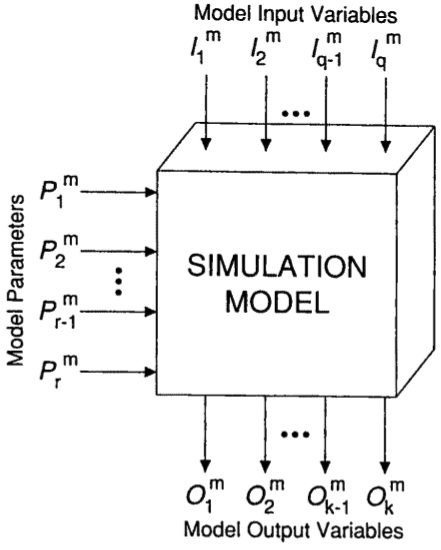
\includegraphics[width=.4\linewidth]{img/Balci1994a_Figure_Parametres.png}
		\caption{Les variables d'un modèle de simulation selon Balci \autocite[122]{balci_validation_1994-2}.\\
		\textit{Nota bene} : ce schéma est tronqué, ne présentant que la partie \og modèle de simulation\fg{} alors que celle-ci est mise en mirroir à une partie \og système\fg{} représentant l'empirique.}
		\label{fig:parametres-Balci} 
	\end{figure}
	
	Dans ce schéma et l'article associé, et bien qu'il n'en définisse nulle part explicitement le sens, Balci esquisse la composition d'un modèle de simulation.
	
	\colorbox{pink}{\parbox{0.9\textwidth}{%
			\vskip5pt
			\leftskip5pt\rightskip5pt
			Décrire le schéma de Balci point par point. Faire un schéma pour Treuil, puis introduire les miens en les explicitant complètement.
			\vskip5pt
		}
	}
	
	
	\subsubsection{Paramètres, variables, indicateurs : un essai de définition}
	\label{subsubsec:mes_definitions_params}
	
	Nous considèrerons donc plutôt les paramètres comme le sous-ensemble des entrées, qui peuvent s'exprimer sous forme numérique (excluant donc de fait certaines entrée telles que les configurations spatiales initiales), et que l'on fera varier, aussi bien dans la calibration du modèle que pour l'exploration de scénarios.
	
	
		\colorbox{pink}{\parbox{0.9\textwidth}{%
			\vskip5pt
			\leftskip5pt\rightskip5pt
			Faire un schéma avec organisation des variables/paramètres/entrées/sorties telles que proposée dans ma thèse.
			\vskip5pt
		}
	}



	\begin{figure}[!h]
	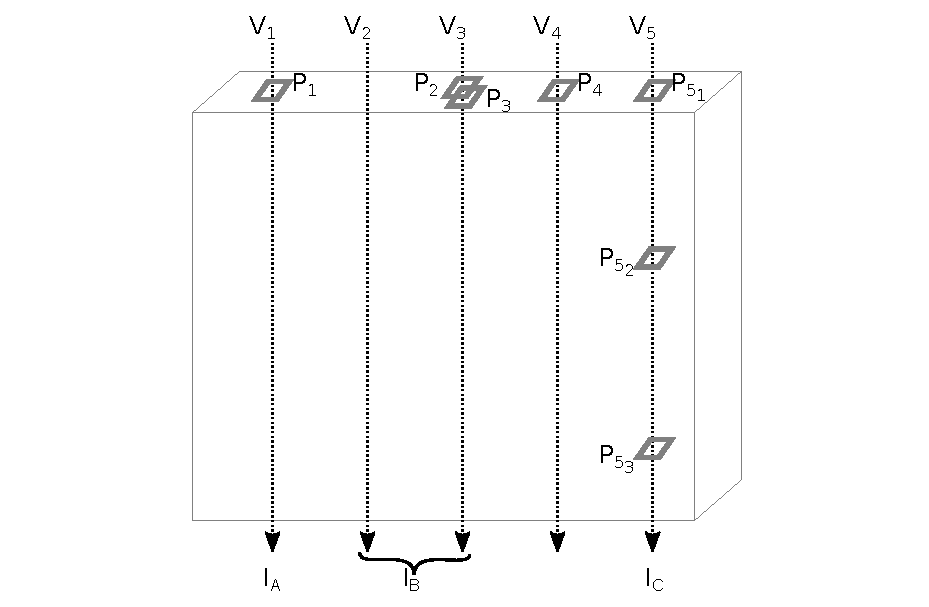
\includegraphics[width=\linewidth]{img/schemas_params_simple.pdf}
	\caption{Schématisation des définitions de variables (V), indicateurs de sortie (I) et paramètres (P).} 
	\label{fig:parametres-these-simple} 
	\end{figure}

	\colorbox{pink}{\parbox{0.9\textwidth}{%
		\vskip5pt
		\leftskip5pt\rightskip5pt
		Ne pas oublier de préciser différence entre paramètres et situation initiale. Ex. de situation initiale : des variables déjà allouées, par ex. pop des villes.
		Il n'y en a pas vraiment dans mon modèle pk tout est endogénéisé : pas de situation initiale, mais des paramètres qui définissent la création de celle-ci.
		\vskip5pt
	}
}

	\begin{figure}[!h]
	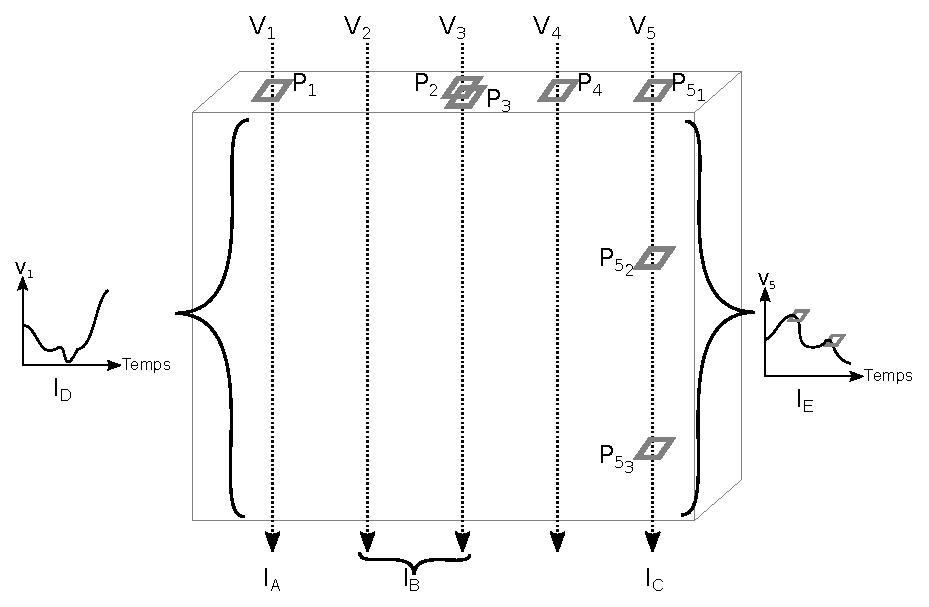
\includegraphics[width=\linewidth]{img/schemas_params_complet.pdf}
	\caption{Schématisation des définitions de variables (V), indicateurs de sortie (I) et paramètres (P) incorporant l'aspect temporel de certains indicateurs ($\text{I}_{\text{D}}$ et $\text{I}_{\text{E}}$).} 
	\label{fig:parametres-these-complet} 
	\end{figure}
	
	\newpage
	\subsubsection{Paramètres et variables}
	
	\begin{encadre}{Variables, entrées, paramètres\ldots}{termes-variables}
		Au sein des \textbf{variables}, constituées par l'ensemble des éléments d'un modèle ayant la capacité de changer, que ce soit au cours d'une simulation ou au travers de plusieurs expérimentations, nous distinguerons trois types spécifiques.
		\begin{description}[style=nextline]	
			\item[Entrées] Les \textbf{entrées} constituent l'ensemble des informations nécessaires à l'exécution d'un modèle en ce qu'elles en alimentent les mécanismes. Elles peuvent être constantes au cours d'une simulation (la date de fin d'exécution de notre modèle par exemple), ou évoluer de par l'action du modèle (le nombre d'églises paroissiale du modèle, qui est une entrée, et augmente tout au long de la simulation).
			
			\item[Paramètres] Certaines de ces entrées sont des \textbf{paramètres} : ce sont les entrées qui peuvent être mobilisées afin de modifier le comportement du modèle, et qui \og représentent ce que le simulateur peut perturber\fg{}\footnote{Pour reprendre les mots de Treuil et al. qu'ils appliquent aux entrées\autocite[8]{treuil_modelisation_2008}. }. Dans cet ouvrage, nous distinguerons plusieurs types de paramètres (\cref{enc:types-parametres}) selon leur ancrage dans l'empirique. Notons toutefois dès maintenant que le nombre de paramètres d'un modèle peut être bien supérieur au nombre de paramètres que l'on fera réellement varier dans les expérimentations.
			
			\item[Sorties] \hl{Les sorties d'un modèle représentent ce que l'on va observer après l'exécution du modèle afin d'observer son déroulement et aboutissement}.\footnote{Pas clair}.
			Ces sorties peuvent être très nombreuses, et concerner autant les variables individuelles (une liste des Foyers Paysans et de leur satisfaction au cours du temps par exemple) que des variables agrégées (Quartiles de satisfaction des foyers paysans par exemple), moins coûteuses en temps d'écriture ainsi qu'en espace de stockage. De la même manière que pour les paramètres, sur l'infinité potentielle de sorties d'un modèle, seules quelques-unes seront effectivement générées et enregistrées afin de minimiser les données produites à celles que le modélisateur compte explorer.
		\end{description}
	\end{encadre}
	
	\subsubsection{Différents types de paramètres}
	
	
	Les paramètres sont donc un sous-ensemble des entrées d'un modèle qui ont vocation à varier dans les différentes exécutions de ce modèle. Pour autant, c'est un sous-ensemble assez divers, et tous les paramètres n'apportent pas les mêmes connaissances, que ce soit par leur valeur ou par la manière dont ils varient. Il convient donc d'identifier différents types de paramètres, non selon leur caractéristique propre (c'est-à-dire leurs propriétés, qui permettent de les différencier des sorties par exemple), mais selon leur usage et donc la manière dont on pourra les mobiliser. A ce titre, quand la littérature en sciences humaines et sociales\footnote{En physique ou en mathématiques par exemple, une telle distinction n'existe pas, la définition d'un paramètre prenant une considération plus simple d'élément rendu constant dans une exécution d'un modèle. \hl{pas clair, prendre une définition quelconque reprenant cette idée.}} distingue souvent (\hl{refs}) deux types de paramètres : les paramètres empiriques, dont la valeur a une correspondance directe dans le domaine empirique (on peut donc l'observer), et les paramètres techniques\footnote{Mathian et Tannier \autocite{mathian_formalisation_2015} utilisent le terme de paramètre mécanique pour définir ce type de paramètres. Nous trouvons l'usage du mot technique plus approprié, en ce qu'il se différencie plus de l'empirique sur le pan de l'usage qui en est fait. De plus, chaque paramètre, empirique, technique ou autre, a un impact sur les mécanismes du modèle, de par la définition que nous empruntons des paramètres \cref{enc:termes-variables}. Nous préférerons donc ce terme de \og technique\fg{} pour éviter les confusions.}, pour lesquels cette correspondance n'existe pas. Comme dans la plupart des typologies ayant trait à la catégorisation de valeurs numériques, de nombreux paramètres peuvent se trouver à l'interface de ces deux classes. Nous en proposons donc une troisième, que nous avons choisi de nommer \og paramètres commensurables\fg{}\footnote{
		La définition du dictionnaire \og Le Petit Robert\fg{} pour ce terme est celle-ci :  \og  Se dit d'une grandeur qui a, avec une autre grandeur, une commune mesure.\fg{}\autocite{robert_nouveau_1993}. \\Cf. aussi :			
		\og Les mondes n'apparaissent commensurables ou incommensurables qu'à ceux qui s'attachent aux mesures mesurées. Or, toutes les mesures, en science dure comme en science souple, sont aussi des mesures mesurantes et celles-là construisent une commensurabilité qui n'existait pas avant leur mise au point.\fg{}\autocite[153]{latour_nous_2013}},
	qui nous semble à même caractériser des paramètres partiellement inscrits dans l'empirie, c'est-à-dire sans valeur empirique propre, mais permettant tout de même d'être mobilisés comme les paramètres empiriques, c'est-à-dire à même d'être comparés, que ce soit par les fluctuations de leurs propres valeurs ou en comparant des paramètres commensurables les uns avec les autres. Avec cette typologie des paramètres basées non sur la nature de ceux-ci mais sur leur utilisation dans un modèle, nous nous inscrivons dans une vision fonctionnaliste et donc très subjective, rappelant la définition d'un modèle de Minsky\footnote{\hl{Cf. sans doute le chapitre 1, à faire.}} \autocite{minsky_matter_1965}. Pour différents modélisateurs, un même paramètre pourra donc être considéré comme empirique ou commensurable, ou encore comme commensurable ou technique.
	\colorbox{pink}{\parbox{0.9\textwidth}{%
		\vskip5pt
		\leftskip5pt\rightskip5pt
			Ne pas oublier de préciser que selon le point de vue du modélisateur, un paramètre peut passer de empirique à commensurable, ou de commensurable à technique (et vice-versa), mais pas \og franchir\fg{} toutes les catégories.
			\vskip5pt
		}
	}
	
	
	\begin{encadre}{Trois types de paramètres}{types-parametres}
		
		\colorbox{pink}{\parbox{0.9\textwidth}{%
				\vskip5pt
				\leftskip5pt\rightskip5pt
				Regarder s'il y a des enquêtes sur les seuils de satisfaction de Schelling dans la littérature.
				\vskip5pt
			}
		}
	
		\begin{description}
			\item[Paramètres empiriques] Les paramètres empiriques sont les paramètres qui peuvent être fixés à l'aide d'une ou de valeur(s) empiriquement connue(s), ou à défaut, dont la valeur se réfère à une quantité directement identifiable par une personne ayant des connaissances thématiques sur ce qui est modélisé.
			\begin{mdframed}[backgroundcolor=gray!10,footnoteinside=false]
				Dans le modèle de Schelling (\ref{desc:schelling}), le paramètre \fixref{\texttt{S}} est un paramètre empirique : la valeur qui lui est donnée peut être interprétée empiriquement, quand bien même il serait difficile d'obtenir, par exemple d'un enquêté, une valeur exacte à utiliser.
			\end{mdframed}
			\item[Paramètres techniques] Il s'agit des paramètres dont la valeur, ou même son ordre de grandeur, n'apportent aucune connaissance thématique au modélisateur. Ces paramètres ont pour raison d'être de permettre à d'autres types de paramètres de s'exprimer en valeurs compréhensibles et exploitables. Dès lors, leurs valeurs sont propres à chaque modèle formalisé, et une comparaison de ces valeurs entre les différents modèles n'apporte pas de connaissance.
			
			\begin{mdframed}[backgroundcolor=gray!10,footnoteinside=false]
				Dans le modèle gravitaire (\cref{desc:gravitaire}), $k$ est un paramètre technique : c'est un ratio qui varie afin d'ajuster l'ordre de grandeur des masses ($M_i$ et $M_j$) à celui des flux  échangés ($F_{ij}$). C'est une valeur d'ajustement, qui ne peut être comparée entre des modèles portant sur différents espaces et/ou thématiques\footnotemark.
			\end{mdframed}
			
			\item[Paramètres \og commensurable \fg{}]
			
			Cette catégorie, forgée dans le cadre de cet ouvrage, permet de représenter les paramètres qui ne sont pas fondamentalement issus de l'empirique mais qui peuvent toutefois être interprétés, que ce soit par rapport à une valeur canonique, définissant alors un repère, ou alors par rapport à d'autres valeurs de ce même paramètre, créant dès lors une échelle d'analyse. Outre la calibration d'un modèle, les valeurs de ces paramètres ont donc un intérêt propre et peuvent être analysées. pour elles-mêmes.
			
			\begin{mdframed}[backgroundcolor=gray!10,footnoteinside=false]
				Dans le modèle gravitaire (\cref{desc:gravitaire}), le frein de la distance (paramètre $\alpha$) peut être considéré comme un paramètre commensurable. Sa valeur ne renvoit ainsi à aucune dimension empirique, mais son usage répandu permet de comparer les valeurs qu'il peut prendre à des valeurs bien connues. Par exemple, on utilise fréquemment des valeurs de $\alpha$ comprises entre $1$ et $2$ pour exprimer la friction de la distance dans les navettes domicile-travail. Une valeur inférieure à $1$ peut donc être interprétée comme laissant une part plus faible à la distance, par exemple dans le cas de déplacements de loisirs. A contrario, un paramètre $\alpha$ supérieur à $2$ montrera une plus forte friction de la distance, par exemple dans les choix d'une école élémentaire à proximité du foyer d'un ménage.
			\end{mdframed}
		\end{description}
		\footnotetext{Dans le cas où $\alpha$ vaut $0$, ce paramètre peut être vu comme commensurable dans la mesure où il devient alors la part de la masse qui devient un flux.}
	\end{encadre}
	
	
	\subsubsection{Comment choisir les valeurs de paramètres ?}
	
	\hl{Ici, faire un court paragraphe de transition pour présenter rapidement l'approche générale du paramétrage : peut-être redondant avec ce qui suit, en particulier dans les présentations des paramètrages du modèle gravitaire et de Schelling.}
	
	\subsection{Le paramétrage, un processus d'amélioration du modèle.}
	
	Le paramétrage d'un modèle est souvent réduit à l'un de ses aspects, le \og calibrage \fg, étape finale de la construction d'un modèle qui cherchera à reproduire autant que possible des données empirique en faisant varier les valeurs des paramètres jusqu'à ce qu'une combinaison de celles-ci soit satisfaisante.
	
	De nombreux auteurs ont montré que le paramétrage d'un modèle ne pouvait se réduire à cette étape, chacun employant des termes différents pour désigner le processus de paramétrage.
	
	%%%% Pas adapté  %%%%
	Gilbert et Troitzsch \autocite{gilbert_simulation_2005} restent très flous en utilisant les termes de \textit{checking} et de \textit{debugging}, qu'ils inscrivent dans une démarche plus large de \textit{verification} correspondant à la \hl{validation interne}\footnote{\hl{Définir !}}.
	Osman Balci \autocite{balci_validation_1994-2} crée et emploie l'acronyme \og \textit{VV\&T}\fg{}\footnote{\textit{Validation, Verification and Testing}}, à portée plus large puisqu'il s'applique à chacune des étapes de la modélisation
	%%%%  %%%%
	
	Le plus souvent (\fixref{ref Seb, Clem...}), une fois le modèle construit, le modélisateur s'attache à son \og calibrage\fg{}, en cherchant pour chaque paramètre la ou les valeurs qui permettront au modèle de s'approcher des données empiriques devant être reproduites.
	Cette étape, que l'on nomme généralement calibration, peut se faire de manière manuelle, par approximations successives (\fixref{C. Cottineau et/ou S. Rey, d'après Hermann}), par semi-automatisme, \change{Lena : trouver d'autres exemples plus classiques et lointains}{exemple en effectuant des analyses de sensibilité} (\fixref{C. Schmitt, J. Hirtzel}), ou encore de manière entièrement automatique (\fixref{C. Schmitt, S. Rey, C. Cottineau avec PSE}).
	L'approche souvent défendue, notamment dans les travaux les plus récents (\fixref{Rimbault?}), voudrait que cette étape soit obligatoire pour toute modélisation, permettant par une exploration systématique de comprendre l'entièreté du comportement d'un modèle, et d'en faire dès lors un outil complètement maitrisé \change{Lena: expliciter}{rendant possible l'établissement d'une loi}.
	
	Dans notre travail, nous souhaitons revenir sur cette approche de la modélisation, ancrant le paramétrage comme étape ultime de la construction d'un modèle, en particulier en ce que nous considérons que cette pratique de recherches de \change{Lena : penser à bien l'introduire avant.}{valeurs optimales} est un exercice qui devrait s'effectuer tout au long de la construction du modèle, de manière plus itérative que conclusive.
	
	
	\subsection{Qu'est-ce que le(s) paramétrage(s) ?}
	
	\subsubsection{Définition}
	
	\change{J'aime bien cette définition, c'est la seule à avoir le sens que j'entends dans paramétrage/paramétrer. Et elle introduit une logique d'optimalité.}{Paramétrer (informatique): \og Programmer (un appareil complexe), en définissant les paramètres assurant son fonctionnement optimal. Ex. \textit{Paramétrer une imprimante}\fg{}\autocite{robert_nouveau_1993}.}
	
	Le terme recouvre deux sens différents, dont la distinction peut se faire selon qu'on l'utilise pour définir un processus ou pour caractériser une configuration.
	Ici, nous emploierons plutôt le premier cas, définissant dès lors le paramétrage comme le processus, manuel ou automatique, visant à constituer cette configuration de paramètres.
	Dans ce deuxième cas, le paramétrage désigne un ensemble de valeurs de paramètres, par exemple quand on mentionne un paramétrage par défaut, ou un paramétrage optimal.
	Pour ne pas risquer de contre-sens, nous préférerons le terme de configuration de paramètres.
	
	On tend à distinguer le paramétrage -- passage obligé ne nécessitant pas d'être évoqué -- de la calibration, processus systématique qui inscrirait le modèle comme un outil scientifique et incontestable.
	Nous choisissons ici de confondre ces approches, non pas en considérant le paramétrage comme un outil d'évaluation du modèle, mais comme une composante inhérente à la construction d'un modèle, quelque soient les formes et les temporalités que le paramétrage adopte.
	Le paramétrage est en effet une pratique utile dans la construction du modèle, car les résultats auxquels il aboutit, c'est-à-dire les valeurs de paramètres qui semblent mieux adaptés, renseignent aussi bien sur les biais des mécanismes adoptés que sur leur efficacité réelle.
	Par exemple, quand, après avoir ajouté un mécanisme, on se rend compte que des variations dans les valeurs de paramètres ne changent pas réellement les sorties du modèle, cela peut être l'occasion de repenser le mécanisme dans son ensemble, ou plus souvent, la manière dont le paramètre est mobilisé dans ce mécanisme. On retrouve cette logique dans l'exploration par Clara Schmitt du modèle SimpopLocal \autocite{schmitt_modelisation_2014-1}, qui a permis de réaliser que la variation de l'un des paramètres ($InnovationLife$) n'avait que peu d'impact sur les sorties du modèle, tout en rendant sa calibration plus complexe et instable :
	\begin{quote}
		Au dessous du seuil des 150 pas de simulation pour le paramétrage de InnovationLife, le calibrage du modèle est très difficile voire impossible. Au dessus de ce seuil, le mécanisme associé au paramètre InnovationLife n’a plus d’effet sur le calibrage du modèle. Dans un soucis de parcimonie du nombre et de la complexité des mécanismes simulés dans le modèle SimpopLocal, il est justifiable de retirer du modèle ce mécanisme qui n’est pas nécessaire à la simulation de la dynamique de croissance recherchée.\\
		\mbox{}~ \hfill \autocite[224]{schmitt_modelisation_2014-1}
	\end{quote}
	
	\paragraph{}Afin d'illustrer ces propos, on peut s'appuyer sur des modèles bien connus de la littérature, issus de deux champs disciplinaires différents.
	
	\subsubsection{Illustration : le modèle gravitaire.\label{desc:gravitaire}}
	
	\paragraph{Description}	Ce modèle statistique\footnote{Pour une description plus complète, se référer à l'ouvrage de Pumain et Saint-Julien \autocite{pumain_les_2001}.}, dans la formulation qu'en a faite Stewart \autocite{stewart_demographic_1948}, vise à prédire des flux (démographiques, marchands etc.) potentiels entre des lieux à partir d'une analogie avec la loi physique de la gravitation. Dans le formalisme le plus simple, \og sans contrainte\fg{} \autocite{pumain_les_2001}, on peut l'exprimer ainsi :
	$$
	F_{ij} = \frac{k \times M_{i} \times M_{j}}{d_{ij}{}^\alpha}
	$$
	Ce modèle présente trois valeurs empiriques ($M_i$, $M_j$ et $d_{ij}$) et deux paramètres ($k$ et $\alpha$). $k$ est un paramètre technique (\cref{enc:types-parametres}), puisque bien que basée sur l'empirique, sa valeur -- et les fluctuations de celle-ci -- ne donne aucune information sur le système étudié. $\alpha$ est un paramètre commensurable pour les raisons explicités dans l'\cref{enc:types-parametres}.
	
	À partir des valeurs empiriques $M_i$ et $M_j$ qui caractérisent les masses (populations, ou stocks de  marchandise par exemple) des lieux $i$ et $j$, et de la distance qui les sépare $d_{ij}$, on peut ainsi prédire $F_{ij}$, le flux entre ces lieux.
	
	\paragraph{Objectif} Afin que ce modèle donne des ordres de grandeur réalistes quand aux quantités échangées, il faut le paramétrer en définissant une valeur de $k$, permettant dès lors d'obtenir un rapport entre les masses d'origine et les quantités échangées.
	La valeur de ce paramètre est conditionnée par celle de $\alpha$, que l'on nomme fréquemment \og frein de la distance\fg{}, en ce qu'il permet de quantifier l'impact qu'aura un éloignement plus ou moins important sur la quantité de flux échangés.
	
	\paragraph{Paramétrage} Pour \og ajuster\fg{}\footnote{C'est le terme employé par \autocite{pumain_les_2001}, que l'on peut ici retenir comme équivalent de paramétrer. François Durand-Dastès  \autocite[298]{durand1995modeles} utilise pour sa part le terme de calibration à propos du même modèle.} le modèle, il faut donc en réaliser le paramétrage en s'appuyant sur les éléments connus de l'équation (les valeurs empiriques).
	$\alpha$ et $k$ étant liés dans l'équation, la valeur de chacun de ces paramètres dépend de celle choisie pour l'autre, et un changement dans l'un des paramètres entraînera la nécessité de modifier l'autre.
	
	Le paramétrage le plus simple consiste à réaliser une régression linéaire sur les logarithmes décimaux des distances et des flux observés, $k$ prenant alors la valeur du logarithme de l'ordonnée à l'origine et $\alpha$ celle du coefficient directeur de la courbe.	
	Le modèle est alors calibré (voir \cref{enc:termes-calibration}), mais si l'on souhaite donner une valeur spécifique à l'un des paramètres, par exemple pour utiliser une valeur classique de 2 au frein de la distance ($\alpha$) \autocite{pumain_modegravitaire_2004}, il faudra alors le re-soumettre à paramétrage pour adapter $k$. De même si l'on modifie les lieux et/ou les masses sur lesquels il s'applique.
	
	
	\subsubsection{Illustration : le modèle de ségrégation de Schelling.\label{desc:schelling}}
	
	\paragraph{Description}Le modèle de Schelling\footnote{Une description plus poussée accompagnée d'une description de l'exploration du modèle peut être lue dans \autocite{daude_comparaison_2006}} est un modèle de simulation décrit par Thomas Schelling \autocite{schelling_dynamic_1971} qui vise à montrer comment un espace peut passer d'un état intégré à un état ségrégé ethniquement à travers une succession de comportements individuels de mobilité résidentielle. Il montre en particulier qu'on peut parvenir à un état ségrégé même quand les comportements individuels sont majoritairement tolérants.
	
	L'espace du modèle est défini comme une grille carrée composée de $N$\footnote{Nous reprenons ici la notation $M(N, d, n, S)$ proposée par \autocite[433]{daude_comparaison_2006} en n'explicitant toutefois pas le paramètre $n$ décrivant le type de voisinage (4 ou 8) utilisé.} cellules.
	Au début de la simulation, des agents de deux types, en proportions similaires, sont distribués aléatoirement dans l'espace du modèle. Chaque agent occupe une cellule, et le nombre total de cellules occupées (et donc d'agents) dépend d'un paramètre de densité $d$ qui représente la part (entre $0\%$ et $100\%$) du nombre de cellule qui sera occupé\footnote{Il y a donc $N \times d$ agents, et donc $\frac{N \times d}{2}$ agents de chaque type.}.
	Chaque agent est défini par une satisfaction. Celle-ci correspond à la part de cellules voisines occupées par des agents \og étrangers\fg{}, c'est-à-dire d'un autre type : plus le voisinage contient d'étrangers, moins l'agent est satisfait.
	Si cette satisfaction est inférieure à un paramètre de tolérance $S$, l'agent est considéré comme insatisfait et se déplace aléatoirement dans une cellule non occupée.
	A terme, Schelling montre que même en considérant des valeurs de $S$ assez élevées, c'est-à-dire un comportement plutôt tolérant, la succession de choix individuels entraîne la mise en place d'une distribution spatiale très ségrégée.
	On considère que le modèle a convergé quand l'ensemble des agents sont satisfaits, ce que ne permettent pas toutes les combinaisons de valeurs de paramètres.
	
	Dans ce modèle, on peut donc dénoter trois paramètres, $N$, $d$ et $S$. Les deux premier sont des paramètres techniques (\cref{enc:types-parametres}), en ce que, purement théoriques, ils ne se réfèrent à aucune quantité empirique, ni ne peuvent être utilisés afin de se référer à un ordre de grandeur connu qui en ferait des paramètres commensurables. $S$ est un paramètre empirique. Bien que le modèle soit théorique, ce paramètre se réfère toutefois à une comportement ayant un sens empirique fort.
	
	\paragraph{Objectif} Le paramétrage de ce modèle consiste à fixer un $N$ constant et à faire varier $d$ et $S$ afin d'en trouver des valeurs permettant la convergence vers une situation stable. Quand $d$ est très faible ($30\%$ dans l'exemple de \autocite{daude_comparaison_2006}), quelles que soient les valeurs de $S$, le modèle converge rapidement : quand l'espace du modèle dispose d'une faible densité d'agents, il est facile pour ceux-là de créer des agrégats homogènes distants d'agrégats de l'autre type d'agents. Quand $d$ est plus important ($\geq66\%$), l'espace disponible étant limité, toutes les valeurs de $S$ ne permettent pas la convergence du modèle. Le paramétrage du modèle aura donc pour objectif de trouver la valeur maximale possible -- pour un $N$ et un $d$ donné -- que peut prendre le paramètre de tolérance $S$ tout en laissant le modèle converger.
	
	\paragraph{Paramétrage}Contrairement au modèle gravitaire, le modèle de Schelling est stochastique : les agents se déplacent aléatoirement quand non satisfaits. Dès lors, deux exécutions du modèle avec le même jeu de paramètres n’entraîneront pas forcément la même configuration spatiale. Qui plus est, pour certains jeux de paramètres, seules certaines exécutions convergeront. Le paramétrage de ce modèle ressemble donc à celui qui est réalisé pour le modèle SimFeodal. La manière \og traditionnelle\fg{}\footnote{C'est-à-dire manuelle, au contraire de méthodes automatiques plus rigoureuses et récentes.} consiste à fixer un $d$, puis à essayer d'augmenter le $S$ tant que le modèle converge. Si le modèle converge pour tout $S$, on augmente la valeur de $d$ et on recommence à chercher la valeur maximale possible pour $S$. De part la nature stochastique du modèle, chaque jeu de paramètres doit être simulé plusieurs fois, le nombre de ces réplications dépendant de la part d'aléa dans le comportement du modèle.
	Un modèle de Schelling calibré, c'est-à-dire dont le paramétrage est achevé,
	donnera pour un $N$ fixé les valeurs maximales de $d$ et de $S$ atteignables.
	
	\paragraph{}A travers ces deux exemples ayant traits à des méthodes différentes, on retrouve deux approches de paramétrage que l'on souhaite ici voire confondues : dans le premier cas, le paramétrage du modèle gravitaire tend à sa calibration, à la recherche d'une solution optimale, c'est-à-dire meilleure que toute autre. Pour un phénomène donné (un jeu de données précis par exemple) et un formalisme donné (l'expression la plus simple du modèle, ici sans contrainte), seule un couple de paramètres $\alpha$ et $k$ permet ainsi d'obtenir des flux modélisés proches des flux observés.
	Dans le cas du modèle de Schelling, il n'y a pas de recherche d'optimum : le paramétrage permet de comprendre le modèle en en définissant les limites en matière de convergence. Une configuration de paramètres $S$ et $d$ ne sera pas meilleure qu'une autre, mais pour un $S$ donné, on saura quel est la valeur maximale de $d$ permettant cette convergence (et réciproquement).
	
	\subsubsection{Paramétrer un ou des modèles ?}
	
	\change{Lena : trop endogame, prendre exemples modèles modulaires dans JASSS}{\fixref{Cottineau, Reuillon et Rey} ont montré qu'on construisait plus souvent des familles de modèles que des modèles uniques.}
	Ces auteurs plaident pour une construction modulaire de modèles, chacun des mécanismes et complexifications devant être autonomes afin de pouvoir les assembler en autant de combinaisons que nécessaire à une exploration d'ensemble de leurs interactions.
	
	Nous reprendrons de leur discours une vision moins ambitieuse, en considérant (\changec{ref Rey}{à chercher il en parlait à sa soutenance je crois}) simplement qu'en fait d'un modèle, la modélisation passe par plusieurs modèles, ayant chacun différentes implémentations d'un mécanisme conceptuellement identique et chacun se devant dès lors d'être adapté par un paramétrage dédié.
	
	Pour illustrer ce propos, on peut prendre l'exemple d'une modification qui a eu lieu sur notre modèle au cours de son développement. On considérait jusque là que pour prendre en compte la population rurale (hors Tours donc), $1000$ foyers paysans donnaient une bonne idée de la situation en 800 pour l'espace considéré.
	Lors d'une réunion, les thématiciens se sont rendus compte que ce nombre sous-estimait très largement la population réelle, et qu'il valait mieux passer ce paramètre à $4000$ foyers paysans.
	Les autres paramètres, fixés en bonne partie empiriquement, n'avaient visiblement aucune raison d'évoluer du fait de ce changement. Les mécanismes  et effets de seuil étaient en effet conçus de manière à être relatifs aux masses manipulées, et le changement attendu était une augmentation linéaire des indicateurs de sortie.
	
	\begin{figure}[H]
		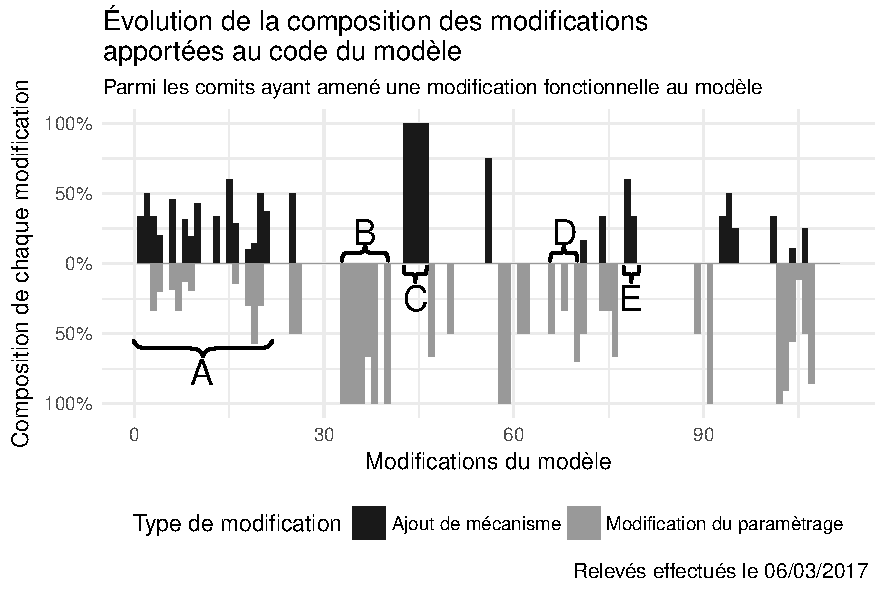
\includegraphics[width = \linewidth]{img/plotComits.pdf}
		\caption{Temporalité du paramétrage du modèle.\\
			Chaque \og enregistrement\fg{} (\textit{comit}) correspond à une version modifiée et sauvegardée du modèle, contenant un ou plusieurs changements. On a ici rapporté le nombre de changements de chaque type (modification de mécanisme ou de valeur de paramètre) au nombre total de changements de chaque \textit{comit} afin de figurer l'évolution des types de modification au cours de la construction du modèle.}
		\label{fig:comits-periodes}
	\end{figure}
	
	Dans les faits, cette légère modification a entraîné une obligation de repenser la quasi-totalité des autres paramètres et d'ajuster une bonne part des règles. 
	La concentration des foyers paysans était en effet bien trop rapide avec autant d'individus, et le modèle convergeait en quelques pas de temps vers une configuration presque statique et très concentrée.
	Tous les mécanismes de régulation de ce comportement étaient dès lors rendus ineptes, et il a fallu changer en profondeur la manière dont chaque paramètre et mécanisme interagissait avec les autres.
	\change{Lena : Là on ne suit pas, mais ce sera explicité dans le chap. 2}{C'est un changement majeur, que l'on peut constater dans la figure~\ref{fig:comits-periodes} (1ère modification de la période B), ayant donc entraîné des adaptations de tous les plans du modèle (paramètres en B, mécanismes en C).}
	La première version avait été paramétré aussi correctement que possible, mais ce paramétrage était entièrement à refaire avec la nouvelle version (modifications de la période B, \cref{fig:comits-periodes}).
	\change{Lena : à discuter plus profondément}{On pourrait dès lors différencier le modèle pré-existant et celui qui a suivi ce changement, et les considérer comme deux modèles puisque réagissant de manière extrêmement différente.}
	
	\change{Lena: Pas clair et pas assez logique}{Cet exemple renforce le caractère nécessaire du paramétrage, et qui plus est, de la continuité de cette étape, qui ne peut être pensée que comme une calibration finale d'un modèle abouti, auquel on ne peut en fait parvenir que par des paramétrages réguliers de modèles successifs moins aboutis.}
	
	\subsubsection{Désambiguïsation}
	
	De nombreux termes sont utilisés dans la littérature, souvent sans réelle distinction, pour désigner cette opération qui consister à choisir un jeu de paramètres pour un modèle. Pêle-mêle, on y retrouve le paramétrage, la validation, l'évaluation ou encore la calibration. Nous définissons dans l'\cref{enc:termes-calibration} le sens donné à chacun de ces termes dans le cadre de ce manuscrit.
	\bigskip
	
	\begin{encadre}{Calibration, évaluation, validation\ldots}{termes-calibration}
		\begin{description}[style=nextline]	
			\item[Calibration] On réserve souvent, et nous nous y tiendrons, ce terme à la dernière étape dans l'aboutissement d'un modèle.
			Une fois les mécanismes fixés et des objectifs définis, on peut procéder à la calibration, c'est-à-dire à une exploration de l'espace des paramètres ayant pour but de stabiliser les paramètres afin de se rapprocher autant que possible de ces objectifs.
			Cette étape, quelques soient les moyens employés, s'approche de la résolution utilisée dans le cadre de systèmes d'équations.
			Le contexte des systèmes complexes, et donc d'une non-linéarité des effets des paramètres, rend toutefois difficile l'obtention d'une unique configuration de \hl{paramètres optimale}\footnote{Lena : il faut partir d'une def plus basique en intro}, et la calibration aboutit donc souvent à un ensemble de configurations possibles, constituant par exemple un optimum de Pareto (\fixref{Trouver ref}).
			
			\item[Évaluation] On emploie majoritairement ce mot pour décrire les méthodes permettant de comprendre le comportement du modèle et sa réaction aux différents paramètres.
			Là où la calibration cherche une configuration de paramètres optimale, l'évaluation tend surtout à caractériser la stabilité du modèle face à l'aléa ou a des configurations exceptionnelles.
			On vise ainsi à s'assurer que le modèle reproduise \hl{les faits stylisés}\footnote{Lena : pas introduits avant} voulus quelque soient son réglage, ou au moins à quantifier les intervalles de paramètres qui y satisfont.
			
			\item[Validation] La validation (refs Seb) tire son origine de sciences plus nomothétiques, et correspond donc à la démonstration qu'un modèle reproduit correctement ce qu'il représente. Au delà de l'évaluation, le terme amène une logique de preuve formelle que le modèle réagit bien ainsi et pas autrement quelque soient les conditions d'exécution. Cette démonstration formelle peut être effectuée sur des modèles à faible nombre de paramètres et mécanismes, mais le terme n'est jamais (à vérifier) employé dès lors que les modèles se complexifient.\footnote{Lena : cf. JASSS : Faire un rappel du sens classique, par ex. en stats.}
		\end{description}
	\end{encadre}
	
	
	\subsection{Comment paramétrer ?}
	
	\subsubsection{Visual validation}
	
	(Trouver ref dans thèse Clémentine, sans doute Hermann encore)
	
	\subsubsection{Indicateurs}
	
	\subsubsection{L'importance de la réplication}
	
	\section{Paramétrer ? Quoi et comment ?}
	\subsection{Différents points de vue sur la définition d'un paramètre}
	\subsection{Les paramètres dans les modèles agents}
	\subsection{Le paramétrage, un processus d'amélioration du modèle.}
	\subsection{Qu'est-ce que le(s) paramétrage(s) ?}
	\subsection{Comment paramétrer ?}
	
	
	\clearpage
\section[Évaluer SimFeodal]{Évaluer le modèle SimFeodal}

Le modèle SimFeodal présenté dans le chapitre 2 correspond à une \og version 0\fg{} du modèle souhaité, c'est-à-dire qu'il en constitue une première pré-version -- implémentant l'ensemble des mécanismes décidés dans le modèle conceptuel --, qui n'est pas encore stabilisée dans les liens, interactions et valeurs de paramètres de ceux-ci.
Il ne répond donc pas nécessairement aux attentes que l'on peut en avoir.
Si l'on a déjà mentionné des objectifs dans le chapitre précédent (\hl{ref. à ce passage dans, par ex. tableau, dans cp. 2)}, il convient ici de formaliser et d'expliciter le sens de ces attentes.
En effet, celles-si sont hétérogènes, aussi bien dans leur forme que dans l'importance qui leur est accordée, et la description de leurs caractéristiques se révèle importante pour leur mobilisation dans le cadre du paramétrage -- et de l'ensemble des étapes de la vie d'un modèle -- de SimFeodal.
Dans cette partie, on explicitera donc d'abord le sens que l'on prête à ces attentes, sous la forme d'indices empiriques et d'indicateurs de sortie de simulation.
On présentera alors les méthodes visant à réduire la complexité de ces indicateurs de sortie, proches de ce que se fait en statistiques :
réduction de dimensionnalité et/ou catégorisation et hiérarchisation de ces indicateurs.
En mobilisant les méthodes choisies, on pourra décrire et qualifier le comportement du modèle SimFeodal tel qu'il a été décrit, dans sa version 0, dans le chapitre précédent (\hl{ref à chap 2}).

\subsection{Indices et indicateurs}

On attend d'un modèle, sans entrer encore dans le détail, qu'il reproduise au moins les grands traits de l'élément empirique qu'il cherche à simplifier.
Ces grands traits peuvent s'entendre de multiples manières, et se formaliser avec encore plus d'approches.
Ici, nous avons souhaité proposer une dychotomie simple entre le domaine de l'empirique et celui de la simulation, en forçant et systématisant l'usage d'un vocabulaire qui est souvent employé de manière plurielle.
Pour être en mesure d'évaluer la vraisemblance du comportement empirique reproduit par le modèle, il est nécessaire de s'appuyer sur des éléments empiriques ayant une correspondance dans le modèle de simulation.
Nous caractérisons ces éléments en deux grands ensembles :
(1) \textbf{les indices empiriques}, éléments quantifiables ou au moins descriptibles du domaine empirique, et  (2) \textbf{les indicateurs de sortie}, variables informatiques produites par le modèle de simulation et devant pouvoir être comparés à chacun des indices empiriques.
La \cref{fig:schema_indices} reprend, sous forme de schéma ontologique synthétique, ces ensembles, explicitant le vocabulaire mobilisé dans cette partie.

\begin{figure}[H]
	\captionsetup{width=\linewidth}
	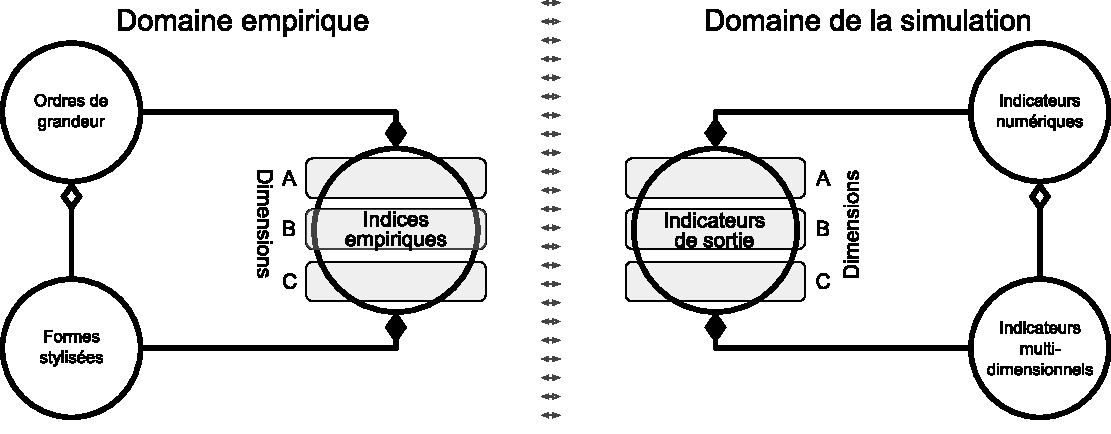
\includegraphics[width=\linewidth]{img/schema_indice_indicateur.pdf}
	\caption{Schéma de synthèse des correspondances entre empirie et simulation pour l'évaluation du modèle SimFeodal.\\
		La correspondance des éléments est représentée par une symétrie axiale.
		Les losanges pleins désignent une relation de composition :
un indice est soit un ordre de grandeur, soit une forme stylisée.
Les losanges vides indiquent une relation d'agrégation :
une forme stylisée est une agrégation d'ordres de grandeurs.
		Les dimensions (A à C) regroupent des indices (et les indicateurs qui leur correspondent) qui peuvent être de plusieurs types, et sont elles aussi comparables et en correspondance entre les domaines.
} 
	\label{fig:schema_indices} 
\end{figure}


\subsubsection{Les indices empiriques}

Le domaine empirique, pour pouvoir être modélisé, doit être en mesure de proposer des \og points de repère\fg{} sur lesquels le modèle s'appuiera.
Ces éléments sont tirés de la thématique des dynamiques que l'on cherche à reproduire.
Selon les modèles, ils peuvent revêtir de multiples formes et caractériser l'ensemble des échelles spatiales et temporelles que l'on choisit de mettre en scène dans le modèle.
Leur point commun est qu'ils doivent pouvoir être mesurés, au sens le plus large, c'est-à-dire être en capacité d'être reproduits et comparables avec d'autres mesures.
Dans cette étude, on a décidé de regrouper ces \textbf{indices empiriques} en deux catégories, basées la précision avec laquelle ils peuvent être décrits\footnote{Et non sur la précision de leur connaissance, cf. \cref{sssec:incertitude}}.
La \cref{fig:schema_indices} montre cette catégorisation entre la première catégorie -- les ordres de grandeur -- et la seconde -- les formes stylisées --.

\paragraph{Ordres de grandeur}
La première catégorie est constituée d'\textbf{ordres de grandeurs} empiriques estimés -- avec une précision plus ou moins importante (\hl{cf. tableau 3 p. 317 du chap. TMD, à reproduire dans chap 2}).
Certaines valeurs empiriques sont ainsi connues, que ce soit d'après des sources primaires ou secondaires, et peuvent ainsi constituer des indices.
Par exemple, on connaît avec quasi-certitude le nombre d'églises paroissiales de la région Touraine en 1100.
Certaines de ces valeurs sont toutefois plus proches de l'estimation, comme le taux de foyers paysans isolés en fin de période, que l'on ne peut qu'estimer à partir de sources secondaires et en menant des extrapolations.
Ces différents indices observés ou estimés peuvent cependant tous trouver une correspondance presque exacte (cf. \cref{para:correspondance}) dans le modèle de simulation, et dès lors, mener à comparaison entre données observées/estimées et données simulées.
Ils peuvent ainsi jouer le rôle d'éléments d'évaluation du comportement du modèle simulé.

\paragraph{Faits et formes stylisés}
Le second type d'indice est moins précis, ne reposant pas sur une valeur estimable, mais plutôt sur la connaissance experte d'un phénomène.
Il s'agit des \og \textbf{faits stylisés}\fg{}\footnotemark{}, plus tendanciels que les indicateurs.
On fait un large usage de ces faits stylisés en économie, mais aussi en géographie, par exemple quand observe que les systèmes de peuplement tendent à se hiérarchiser.
On peut quantifier cette observation en observant que la pente formée par leur courbe rang-taille tend vers $1$ à mesure que le système évolue (\hl{Trouver ref, sans doute Pumain/Saint-Julien}).
De la même manière, le modèle de transition démographique d'Adolphe Landry est un fait stylisé, énoncé à partir de l'observation de nombreuses récurrences de l'évolution des populations d'un pays en fonction des taux de natalité et de mortalité.
Ces exemples montrent qu'au sein des faits stylisés, on retrouve aussi une diversité quant à la précision de leurs énoncés :
on peut quantifier précisément la courbe de la rang-taille et l'allure de son évolution dans le temps, alors que la courbe logistique de la transition démographique revêt un caractère plus théorique.
Dans notre cas d'étude, les faits stylisés sur lesquels on s'appuiera dans la modélisation peuvent être des allures de courbes (par exemple l'évolution dans le temps d'un indicateur) ou encore des formes de répartition spatiale.
On pourra dès lors parler de \og \textbf{formes stylisées}\fg{}, aussi bien temporelles -- courbe logistique estimée pour la polarisation des foyers paysans --, spatiales -- différence dans l'occupation de l'espace par les agrégats entre le début et la fin de la période --, que correspondant à une agrégation à l'échelle du système, comme dans l'observation des hiérarchies grâce aux courbes rangs-tailles.
Notons que ces formes stylisées relèvent le plus souvent d'une agrégation d'ordres de grandeurs (comme figuré dans la \cref{fig:schema_indices}) :
l'évolution dans le temps de la population, par exemple, correspond à un vecteur d'ordres de grandeur, c'est-à-dire à une succession de mesures pour chaque date étudiée.
Dans le cas d'une agrégation spatiale, par exemple quand on observe la hiérarchie du système de peuplement, il s'agit aussi d'une agrégation d'ordres de grandeurs :
cette forme stylisée est constituée d'un ensemble d'ordres de grandeurs, les populations de chaque agrégat de population.

\footnotetext{
	Définis ainsi par \autocite{livet2014diversite}: \og 
	Un ``fait stylisé'' est une présentation simplifiée (i.e. taux, ratio ou écart, structure spatiale) d’une régularité empirique sur l’observation de laquelle il y a un large accord.
Le terme a été popularisé en économie par Nicholas Kaldor (1961).[Les] faits stylisés peuvent être construits de la manière suivante :
1) en partant du domaine empirique, on identifie des relations saillantes ; 2) on opère quelques simplifications qui permettent d’inclure formellement ces relations dans des modèles ; 3) une fois admis que ces simplifications ne faussent pas trop les choses, on érige ces relations à la fois simplificatrices et formalisables au rang de `` faits stylisés'', dont les concepts théoriques doivent rendre compte.\fg{}
}

\subsubsection{Les indicateurs de sortie de simulation}


Les ordres de grandeur et formes stylisées évoquées relèvent du domaine empirique.
Afin de pouvoir les mobiliser, il est nécessaire de définir des \textbf{indicateurs en sortie} dans le modèle de simulation, c'est-à-dire des variables informatiques que l'on enregistrera durant l'exécution du modèle et que l'on pourra ensuite comparer aux indices empiriques définis.


\paragraph{Définition}
Comme pour les indices empiriques qui sont leurs équivalents, on peut définir une typologie différenciant les indicateurs en sortie \og numériques\fg{}, en distinguant les formes numériques simples (des scalaires), et des indicateurs plus complexes, multidimensionnels, à même de permettre la confrontation du modèle de simulation avec les formes stylisées identifiées.
Chaque indice empirique doit ainsi se voir correspondre, respectivement, un indicateur de sortie.

\paragraph{Correspondance entre indicateurs et indices}\label{para:correspondance}

Cette correspondance n'est pour autant pas une équivalence exacte.
En effet, si certains indices empiriques peuvent trouver un équivalent strict -- le nombre de châteaux connus à chaque date est strictement équivalent au nombre de châteaux produits par le modèle --, d'autres indices trouveront une correspondance plus faible.

Il peut s'agir de correspondances ayant trait aux mêmes éléments de bases, donc \og convertibles\fg{} entre elles.
Par exemple, on connaît à peu près les populations de la région étudiée au début et à la fin de la période.
Pourtant, dans SimFeodal, on ne modélise pas les individus en tant que tels, mais des foyers paysans.
Le nombre de foyers paysans simulé n'est pas directement comparable à la population estimée, mais en estimant une moyenne de 4 ou 5 habitants par foyer paysan, ces quantités deviennent équivalentes.

D'autres indicateurs trouveront une correspondance plus lointaine.
Certains indices empiriques ne sont ainsi pas observables directement, et il faut alors leur trouver des indicateurs analogues, que l'on nomme souvent \og proxy\fg{} dans le champs statistique.
Dans notre cas d'étude, il s'agit le plus souvent d'indices plus difficilement quantifiables.
La puissance militaire des seigneurs, par exemple, est complexe à quantifier.
On sait d'après connaissances expertes que la hiérarchie des puissances était forte, majoritairement dominée par deux seigneurs (les comtes de Tours et de Blois) et assortie d'une grande quantité de petits chevaliers.
On sait de plus qu'avec les liens de vassalité, les grands seigneurs disposaient des forces militaires des seigneurs qui leur étaient assujettis.
Faute à une capacité de quantification plus importante de ces indices, on leur associe, dans le modèle, un indicateur proxy relevant du nombre de foyers paysans s'acquittant de droits à chaque seigneur.
De cette manière, on reproduit une hiérarchie implicite entre les seigneurs et leur puissance relative, qui est, elle, comparable aux connaissances empiriques de ces rapports de puissance.

La création d'indicateurs de sortie correspondant aux indices empirique permet donc de quantifier une information qui n'est pas forcément aisément quantifiable dans le domaine empirique.

\paragraph{Indicateur composite}

La forme numérique (scalaire ou vectorielle) des indicateurs de sortie permet de trouver des manières plus simples d'évaluer le modèle que d'observer l'ensemble des indicateurs.
Chaque indicateur étant numérique, il devient en effet possible des les combiner au sein d'indicateurs composites, résultant en quelques indicateurs synthétiques permettant une évaluation plus rapide des résultats d'une simulation.
Ces indicateurs composites sont très fréquemment utilisés en statistiques, permettant par exemple de résumer une information multidimensionnelle en un indicateur simple.
L'Indice de Développement Humain (IDH), par exemple, est un indicateur composite dépendant de l'espérance de vie à la naissance, du niveau d'éducation et du niveau de revenu de chacun des pays caractérisés.
On le trouve très souvent utilisé, parce qu'il permet de résumer le niveau de développement d'un pays en agrégeant trois dimensions majeures, l'aspect sanitaire, culturel et économique.

\paragraph{Indicateur synthétique}

En renforçant cette logique de synthèse de plusieurs dimensions, on peut aller plus loin dans la définition d'un unique indicateur, synthétique, permettant d'évaluer la qualité de représentation d'un modèle.
Là aussi, c'est une pratique très fréquente, qui plus est dans le domaine de la simulation informatique en particulier sur des modèles de type \og KISS\fg{} (\hl{ref. à chap 2 là ou ce sera abordé}).
Il s'agit alors de définir une \og fonction objectif\fg{}, ou \og fonction de \textit{fitness}\fg{}, composée d'une pondération des quelques indicateurs composites qui auront été identifiés.
Être en mesure d'évaluer un modèle à l'aide d'un unique indicateur a des avantages majeurs en pratique, puisque cela permet par exemple d'explorer et de paramétrer un modèle de simulation de manière entièrement automatique (\hl{trouver refs dans JASSS, dans Rey ou Schmitt}) puisqu'on peut alors générer une cartographie simple des résultats du modèle en fonction des valeurs de paramètres utilisés.

Ces indicateurs composites et synthétiques résultent d'une quantification des autres indicateurs (excluant donc les formes stylisées qui sont plus libres d'interprétation), et apportent un grand confort dans le paramétrage d'un modèle de simulation.

\paragraph{Quels types d'indicateurs pour SimFeodal ?}

SimFeodal n'est pourtant pas adapté à de tels indicateurs :
une large partie des faits stylisés et ordres de grandeur mobilisés proviennent de connaissances expertes, et les thématiciens qui les ont consolidées rechignent à créer de tels indicateurs composites, en ce que cela demande de pondérer précisement l'importance de chacun des indicateurs par rapport aux autres.
Pour pouvoir pondérer cette importance, il faudrait de plus que les différents indicateurs mobilisés présentent le même niveau de certitude et de variabilité dans leurs résultats, ce qui est peu le cas des indices empiriques -- et donc des indicateurs de sortie -- choisis dans le cadre du modèle SimFeodal.

On aurait ainsi pu créer quelques indicateurs synthétiques, mais ceux-ci ne prendraient en compte qu'une faible proportion du comportement attendu du modèle, résultant en une forte perte du pouvoir explicatif attendu du modèle.
Par exemple, pour caractériser la polarisation du système de peuplement, il pourrait suffit de définir un indicateur composite fonction du niveau de concentration -- le taux de foyers paysans dispersés --, du nombre de pôles et de l'espacement moyen entre les agrégats.
Les valeurs de l'indicateur généré renseigneraient certes efficacement sur le succès ou l'échec d'un ensemble de valeurs de paramètres, mais cette information serait grossière, agrégeant dans le groupe des \og simulations réussies\fg{} des configurations extrêmement diverses, et donc potentiellement très éloignés des connaissances empiriques :
une information multivariée ne peut pas toujours être résumée de manière univariée.

On a donc fait le choix d'évaluer SimFeodal en conservant des indicateurs de sortie non composites.
Ce choix implique toutefois un problème majeur dans l'analyse des sorties de simulation auquel la réduction de dimensionnalité est une réponse :
il est plus simple d'analyser quelques indicateurs plutôt qu'un grand nombre d'entre eux.
	

\subsection{Hiérarchiser et catégoriser les indicateurs}

SimFeodal s'appuie sur une dizaine d'indicateurs numériques, ainsi que sur plus d'une trentaine d'indicateurs multidimensionnels.
Tous ces indicateurs ne présentent pas le même degré de certitude, la même échelle d'observation, et surtout, le même niveau de précision sur les phénomènes modélisés.
A chaque changement dans le modèle, pour une évaluation complète de la capacité de cette version à reproduire les indices empiriques, il faudrait donc observer et analyser chacun de ces nombreux et divers indicateurs.
Dans le contexte du paramétrage d'un modèle s'appuyant sur une logique itérative et incrémentielle (voir \cref{enc:construction-indicateurs}), on imagine bien que cela n'est pas possible :
le nombre d'indicateurs est bien trop élevé pour avoir rapidement une vision globale de la qualité de représentation du modèle.
Il faut dès lors, comme pour toute analyse synthétique, concevoir une hiérarchie d'observation et d'utilisation des indicateurs :
il ne sera pas nécessaire d'analyser chacun des indicateurs dans la plupart des cas, seuls les indicateurs jugés plus importants pourront être analysés.
Les indicateurs de moindre importance ne seront mobilisés que pour départager des situations dont la différence ne serait pas suffisament explicitée par l'usage des indicateurs principaux.

\subsubsection{Incertitude}\label{sssec:incertitude}
Dans le modèle de simulation, les indicateurs de sortie sont à analyser en tenant compte de la précision des indices qu'ils représentent.
Il ne faudra ainsi pas étudier la croissance  du nombre d'agrégats au cours de la simulation de manière fine, par exemple en étudiant le coefficient directeur de la courbe, quand l'empirie ne donne quasiment aucune information à ce sujet si ce n'est qu'il y a bien plus d'agrégats en fin de période qu'au début.
On peut vouloir quantifier la précision de ces données, par exemple à l'aide des méthodes développées dans le champ des observations floues et/ou incertaines (voir par exemple le travail de Cyril de Runz sur les données \og imparfaites\fg{} \autocite{de2008imperfection}).
Cette quantification de l'incertitude pourrait alors servir de base à l'établissement d'une hiérarchie des indicateurs :
on analyserait en premier lieu l'écart entre les ordres de grandeurs empiriques bien connus (\hl{cf. tableau du niveau de certitude des objectifs}) et les indicateurs calculés sur les données simulées.
Les ordres de grandeur plus incertains seraient analysés dans un second temps (augmentation de la charge fiscale entre 800 et 1100 par exemple), et les formes stylisées viendraient enfin clore cette hiérarchie d'indicateurs.
Toutefois, SimFeodal se caractérise d'une part par une très forte hétérogénéité dans les niveaux de connaissance des ordres de grandeurs et faits stylisés modélisés, et d'autre part, se voulant un modèle théorique (\hl{A dire spécifiquement dans le chapitre 2; y faire une ref ici}), il n'y a pas d'obligation de \og coller aux données\fg{} à tout prix :
la vraisemblance d'ensemble du modèle compte bien plus que la précision de chacune de ses composantes.


\subsubsection{Catégoriser les indicateurs : définir des dimensions d'analyse}
En présence de plus d'une quarantaine d'indicateurs, il est toutefois nécessaire, a minima, d'organiser leur analyse.
On a vu qu'il n'était pas justifié de mener cet ordonnancement à partir des propriétés intrinsèques des indicateurs du modèle.
Au contraire, et cela porte bien plus de sens vis-à-vis du rôle d'un modèle, la hiérarchisation des sortie du modèle doit suivre la hiérarchie implicite qui structure les hypothèses et objectifs du modèle en lui-même.
Ces hypothèses et objectifs sont multiples dans SimFeodal, et dès lors, une hiérarchie globale ne peut être définie.
Il convient donc de catégoriser les indices empiriques -- et les indicateurs de sortie de simulation leur correspondant --, avant d'organiser, au sein même de ces catégories, les indices les caractérisant.
La hiérarchisation des indicateurs se fera donc relativement à chacune de ces catégories.

Dans le chapitre précédent (\hl{ref chap 2}), nous présentions les principales dynamiques à reproduire avec le modèle SimFeodal :
(1) polarisation, (2) hiérarchisation et (3) fixation des foyers paysans.
En postulant que ces dynamiques sont caractéristiques du modèle, on peut s'appuyer sur cette triade pour caractériser les sorties du modèle,c'est-à-dire mener la confrontation entre indices empiriques et indicateurs de sortie.
En reprenant ces catégories, que l'on nommera \textbf{dimensions} (voir \cref{fig:schema_indices}), on va donc répartir chacun des indicateurs dans la dimension qu'il sera le mieux en mesure de décrire.
Cette répartition n'a pas à être égale, chaque dimension pouvant s'appuyer sur un nombre différent d'indicateurs.
De même, chaque dimension sera composée d'indicateurs dotés d'une qualité de représentation ou d'un niveau de certitude hétérogène.
Le seul point commun des indicateurs de sortie de chaque dimension doit être thématique.
Les trois dimensions choisies -- polarisation, hiérarchisation et fixation --, et les indicateurs qui les caractérisent dans le modèle, sont dès lors considérés comme les trois dimensions d'analyse des sorties de SimFeodal.

\subsubsection{Hiérarchiser les indicateurs dans chaque dimension}\label{par:hierarchie_interne}
Chacune de ces dimensions s'applique à plusieurs types d'agents du modèle.
Pour définir la hiérarchie interne aux dimensions, on retiendra les agents les plus impactés par les dynamiques correspondant à ces dimensions :
la polarisation, par exemple, peut être observé depuis le point de vue de ce qui polarise (les attracteurs) tout autant que de ce qui est polarisé (les foyers paysans).
On aura alors tendance à examiner d'abord un indicateur de sortie caractéristique mono-dimensionnel, caractéristique de la structure dans son ensemble à son état final.
Les indicateurs de sortie représentatifs des dynamiques, par exemple les indicateurs multi-dimensionnels, ayant mené à cette structure finale, seront étudiés dans un second temps.
Dans cet exemple, on analysera donc d'abord le résultat effectif de la polarisation, c'est-à-dire la concentration des foyers paysans en agrégats, avant d'observer la répartition et les diversité des attracteurs ayant entrainé ce phénomène.
On peut dès lors définir des \og indicateurs principaux\fg{} pour chaque dimension, représentatifs des grands traits des structures auxquelles on souhaite aboutir en sortie de simulation, et des \og indicateurs secondaires\fg{}, permettant d'affiner l'évaluation de chacune de ces dimensions.

\subsubsection{Une hiérarchie mouvante}
Notons que l'analyse des indicateurs de sortie suit une hiérarchie parfois mouvante, et en tous les cas, assez peu quantifiable :
si l'ordre d'observation est plutôt stable, l'importance que l'on portera à chacun des indicateurs peut varier.
Les indicateurs principaux de chaque dynamique sont ainsi \og incontournables\fg{}, c'est-à-dire qu'un résultat trop loin de celui des indices empiriques est disqualifiant.
Parmi les indicateurs secondaires, il n'est pas toujours possible, d'après les connaissances des experts sur le sujet, d'établir une priorité ou une pondération de chaque indicateur.
L'évaluation de la polarisation par exemple (\cpageref{subsub:polarisation}), se définit principalement par rapport à un indicateur principal -- le taux de foyers paysans dispersés --, mais selon les résultats des autres indicateurs de sortie, on leur attribuera une importance variable.
L'étude de la dispersion des agrégats et pôles peut ainsi se révéler plus importante que celle de l'évolution du nombre d'agrégats selon les paramètres que l'on souhaite ajuster, ou se montrer tout au moins plus différenciante selon l'état du paramétrage.


\begin{encadre}{Incrémentalité des indicateurs}{construction-indicateurs}
	De la même manière que les paramètres et mécanismes d'un modèle de simulation tendent à évoluer\footnotemark{} au cours du temps de la construction, souvent afin d'affiner un comportement observé, les indicateurs de sortie sont amenés à évoluer aussi.
	
	Ainsi, en cas de modifications fines du modèle, il est fréquent que les indicateurs initialement choisis ne suffisent plus à départager des versions du modèle quant à un phénomène spécifique.
Par exemple, quand on observe le phénomène de polarisation dans les sorties de SimFeodal, l'indicateur du nombre d'agrégats est extrêmement synthétique et informatif jusqu'à ce que l'objectif soit atteint ou que les modifications ne parviennent plus à le faire évoluer.
À partir de ce moment, afin d'améliorer la vraisemblance de la situation simulée par le modèle, on peut se focaliser sur la distribution spatiale de ces agrégats, par exemple pour vérifier qu'ils sont bien répartis de manière homogène dans l'espace, et non trop concentrés.
	
L'observation de la répartition spatiale requiert certes de nouvelles analyses, mais surtout, par exemple, d'enregistrer les positions des agrégats au cours du temps.
Si cet indicateur de sortie n'était pas utile avant cela, il n'y avait aucun interêt à l'enregistrer.
Il faut donc adapter l'implémentation du modèle pour générer, faire évoluer et enregistrer une nouvelle variable informatique correspondant à cet indicateur.
Dès lors, on pourra composer un nouvel indicateur synthétique, qui, dans cet exemple, pourrait prendre la forme d'un indice de concentration spatiale).
	
	Ce procédé incrémental dans la construction des indicateurs est très fréquent, mais pose toutefois un problème majeur :
sauf à adapter chacune des anciennes versions du modèle implémenté pour y ajouter l'enregistrement des nouveaux indicateurs nécessaires, on ne pourra rendre strictement comparable les sorties de toutes les itérations du modèles informatique.
Et même alors, il faudrait ré-executer des réplications de chaque version du modèle implementé à chaque ajout d'indicateur, quand bien même les indicateurs présent initialement étaient jugés suffisants.
Un dernier obstacle est plus gênant :
certains indicateurs sont spécifiques à des mécanismes, et en cas de changement de ces derniers, ils peuvent ne plus être calculables ou simplement comparables.
Par exemple, des versions antérieures du modèle enregistraient les comportements individuels des foyers paysans quant à leur \og choix\fg{} de déplacement, selon qu'ils étaient à l'origine localisés dans un agrégat ou dispersés.
Une simplification du modèle a abouti à la modification des règles différenciant les possibilités de déplacement :
on n'observe plus si le foyer paysan est dans un agrégat, mais plutôt s'il est dans un agrégat doté d'un pôle d'attraction.
Dès lors, les analyses basées sur les choix de déplacement des foyers paysans selon leur origine ne sont plus comparables avec celles des versions antérieures au changement dans le modèle, quels que soient les détails d'implémentation de ce dernier.
	
	Ces éléments expliquent que dans les résultats de chaque étape du paramétrage du modèle, on ne présente pas systématiquement l'ensemble des indicateurs, y compris quand ceux-ci pourraient être plus pertinents que les indicateurs présentés.
\end{encadre}
\footnotetext{De manière incrémentielle et itérative, voir \hl{dans le chapitre x?} et http://itsadeliverything.com/revisiting-the-iterative-incremental-mona-lisa}


\pagebreak

\subsection{Les indicateurs et dimensions de SimFeodal}

\subsubsection{Évaluer la polarisation des foyers paysans \label{subsub:polarisation}}

La polarisation des foyers paysans dans l'espace du modèle est sans doute la dimension principale des dynamiques spatiales que l'on cherche à reproduire.
Rappelons ici que l'on estime, à partir des connaissances d'experts, que les foyers paysans sont très majoritairement dispersés en 800, et concentrés au sein de villages et petites villes en 1100.
Le modèle cherche à reproduire cette polarisation, par le biais d'une concentration des foyers paysans, initialement localisés aléatoirement dans l'espace mais n'en parsemant qu'une faible part, en des agrégats de foyers paysans répartis dans dans une plus large partie de l'espace modélisé.
\todobox{Mettre un schéma pour rendre compréhensible cette contradiction apparente.}

Pour analyser la polarisation du système de peuplement, il est nécessaire de définir des indices permettant de caractériser ce phénomène.
Ces indices doivent d'une part avoir une logique thématique, c'est-à-dire être appropriés à la description et à l'étude de la polarisation, mais doivent  pouvoir être produits et enregistrés dans le modèle de simulation, formant des indicateurs.

Pour l'étude de la polarisation, il est nécessaire de faire appel à des indices hétérogènes, chacun devant être en mesure de décrire les différents aspects du phénomène de polarisation.
En conséquence, on a choisi de faire appel à plusieurs indicateurs qui doivent permettre d'étudier aussi bien l'aspect structurel du système simulé en son état final que la forme et la tendance que prennent les changements qu'il subit.

L'indicateur principal est le taux de dispersion des foyers paysans.
Si celui-ci est trop important (c'est-à-dire très supérieur aux valeurs estimées empiriquement), cela signifie que la polarisation générée par le modèle est insuffisante, et dès lors, obligatoirement insatisfaisante.
A contrario, une valeur trop faible serait symptomatique d'un emballement des mécanismes simulés, figeant la situation dans une concentration absolue des foyers paysans, ne laissant dès lors plus de place à la diversification des situations locales et de la hiérarchisation d'ensemble.

Pour affiner ce constat, on fait appel à d'autres indicateurs :
le nombre d'agrégats, de pôles, ou encore la dispersion spatiale de ces deux types d'entités.
Ces indicateurs ne permettent pas, à eux seuls, de caractériser le succès de la dynamique de polarisation modélisée, mais ils aident à affiner l'analyse de cette dynamique telle que produite par le modèle de simulation.
Ils éclairent ainsi le phénomène de polarisation sous des angles légèrement différents, ayant plus pour objet de diagnostiquer les problèmes potentiels qui mèneraient à une mauvaise polarisation plutôt que de qualifier celle-ci.
Par exemple, la dispersion des agrégats et pôles peut renseigner, une fois le taux de foyers paysans dispersé jugé trop important, sur une des raisons probables de ce résultat non satisfaisant.
Il s'agit donc d'indicateurs secondaires, permettant de préciser la capacité du modèle à reproduire les faits stylisés, alors que l'évaluation de cette capacité est surtout le rôle de l'indicateur principal.

\paragraph{Taux de foyers paysans dispersés}

Cet indicateur, et sa déclinaison temporelle, sont vraisemblablement les plus évidents :
plus le taux de foyers paysans dispersés en fin de simulation est faible, plus le système de peuplement est polarisé.
On a vu \footnote{\hl{Ne pas oublier de présenter les objectifs dans chapitre 2. Ou alors, on les présente ici au fur et à mesure qu'on mentionne les indicateurs}} qu'empiriquement, autour de 1160, on observe environ $20\%$ de foyers paysans encore dispersés, alors qu'ils sont près de $95\%$ au départ.
Le modèle sera donc d'autant plus satisfaisant que cet indicateur s'approchera de $20\%$ en fin de simulation.

La \og déclinaison temporelle\fg{} mentionnée juste au dessus permet d'affiner légèrement la précision de l'information communiquée par cet indicateur :
il faut certes atteindre un objectif quantifié ($20\%$), mais les hypothèses empiriques permettent aussi de penser qu'il faut que l'évolution de cet indicateur au cours du temps présente une tendance stable à la diminution, diminuant ainsi plus ou moins, avec de faibles fluctuations à chaque pas de temps.
Une configuration de paramètres présentant des valeurs d'indicateurs en sortie proches des objectifs en fin de simulation mais fluctuant fortement pendant son déroulement ne sera ainsi pas valide.
Elle montrerait en effet  un phénomène trop aléatoire au cours du temps, dont on ne peux penser qu'il s'est déroulé historiquement selon les dires d'experts qui considèrent que cette évolution s'est déroulée de manière continue dans le temps.

\begin{mdframed}[backgroundcolor=gray!10,footnoteinside=false]
	
	Dans la version 0 de SimFeodal, on atteint en moyenne (moyenne des réplications) $\textbf{57\%}$ de foyers paysans isolés en fin de simulation.
	C'est un taux bien plus important que les $20\%$ attendus, illustrant dès lors une polarisation trop faible.
	Dans la première moitiée de la période (jusqu'en 1000, (\cref{fig:taux-isoles-v0})), le taux est en diminution constante et linéaire, ce qui est une bonne tendance, et ne présente de plus presque pas de variabilité, ce qui l'est aussi.
	Pourtant, à partir de 1000, la variabilité augmente, et le la diminution du taux au cours du temps s'interrompt, avant de prendre une allure croissante.
	L'allure de la courbe sur la seconde moitié de la simulation est donc très éloignée de ce qui est attendu au regard des connaissances empiriques, aussi bien en matière de tendance qu'à la vue du taux décevant atteint au final.
\end{mdframed}

\begin{figure}[H]
	\captionsetup{width=\linewidth}
	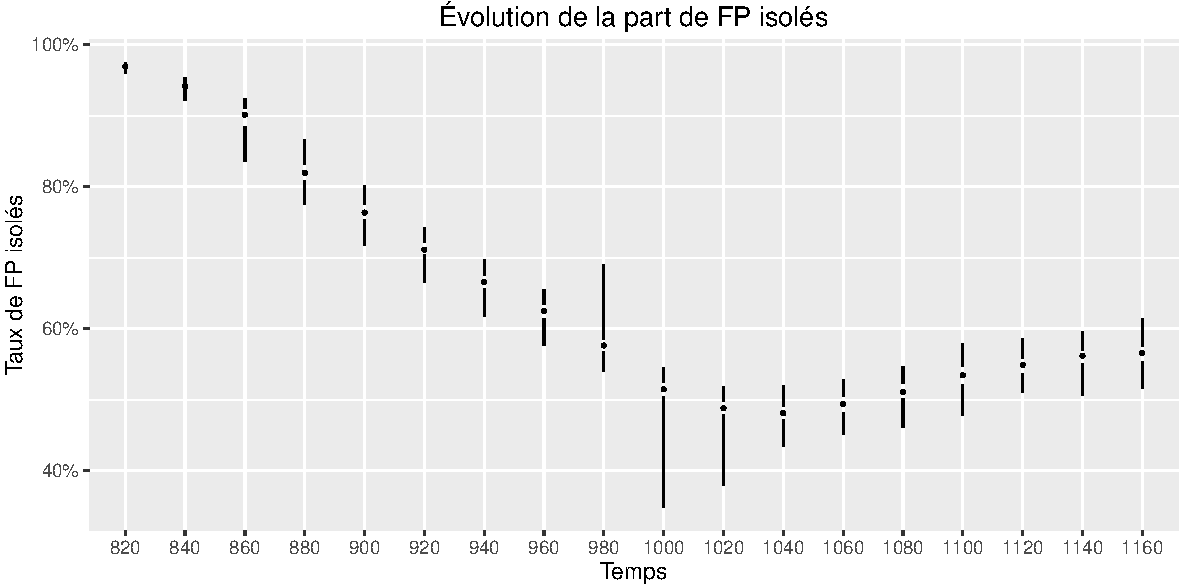
\includegraphics[width=\linewidth]{img/resultats/v0_taux_FP_isoles.pdf}
	\caption{Évolution de la part des foyers paysans isolés.} 
	\label{fig:taux-isoles-v0} 
\end{figure}

\paragraph{Nombre d'agrégats}

Puisque les foyers paysans se concentrent au sein d'agrégats, il est logique d'observer l'évolution de ces derniers.
Là aussi, (\hl{objectif à définir}), on peut considérer qu'un nombre d'agrégats en fin de simulation proche de l'objectif, $200$, permet de caractériser une polarisation réussie.
Cet indicateur ne peut être lu seul, et c'est pour cela qu'il vient dans un second temps (cf. p.\pageref{par:hierarchie_interne}) :
en effet, un faible nombre d'agrégats peut aussi bien être révélateur d'une très faible polarisation des foyers paysans (ceux-ci restant dispersés) que d'une trop importante (un unique agrégat concentrant l'ensemble des foyers paysans par exemple).
Une fois le taux de foyers paysans dispersés connu et ces potentiels biais pris en compte, le nombre d'agrégats et son évolution nous renseigne cependant sur les dynamiques de polarisation.
D'après les connaissances expertes, on s'attend à ce que le nombre d'agrégats, très faible au départ (24 dans la version 0), suive trois phases :
une première phase de croissante lente, le temps que les mécanismes agissent sur la polarisation, suivie d'une période de croissance plus rapide, une fois que tous les foyers paysans commenceront à être suffisament attirés par les pôles pour y former des agrégats, et enfin, une nouvelle phase de croissante plus lente, une fois les foyers paysans répartis dans les agrégats existants et qui se déplaceront vers des agrégats plus importants, hiérarchisant le système de peuplement.
Cette allure d'évolution rappelle les fonctions logistiques connues par exemple pour les cycles de diffusion/adoption des innovations \hl{ref Pumain ou MN Comin}, et résulte des connaissances expertes des archéologues spécialistes de la période.

\begin{mdframed}[backgroundcolor=gray!10,footnoteinside=false]
	Le nombre d'agrégats est assez satisfaisant dans la version 0 du modèle.
Il s'élève ainsi à $\textbf{187}$ en moyenne, cette dernière étant d'ailleurs stable au regard des réplications.
L'écart à l'objectif ($200$) est donc assez minime.
On a toutefois vu que le taux de foyers paysans isolé était bien trop important, et dès lors, ces agrégats sont logiquement composés de trop peu de foyers paysans.
	
	L'observation de cet indicateur au cours du temps (\cref{fig:nombre-agregats-v0}) est quant à elle assez satisfaisante :
on retrouve bien les trois phases attendues, quand bien même le début de la croissance plus importante (vers 1000 ici) est un peu trop tardive.
Ce moment coïncide de plus avec la stagnation puis l'inversion de la courbe d'évolution de la part de foyers paysans isolés.
	
	On peut quand même considérer que si la polarisation n'est pas assez importante, les structures qui en résultent semblent correspondre à l'empirie.
\end{mdframed}

\begin{figure}[H]
	\captionsetup{width=\linewidth}
	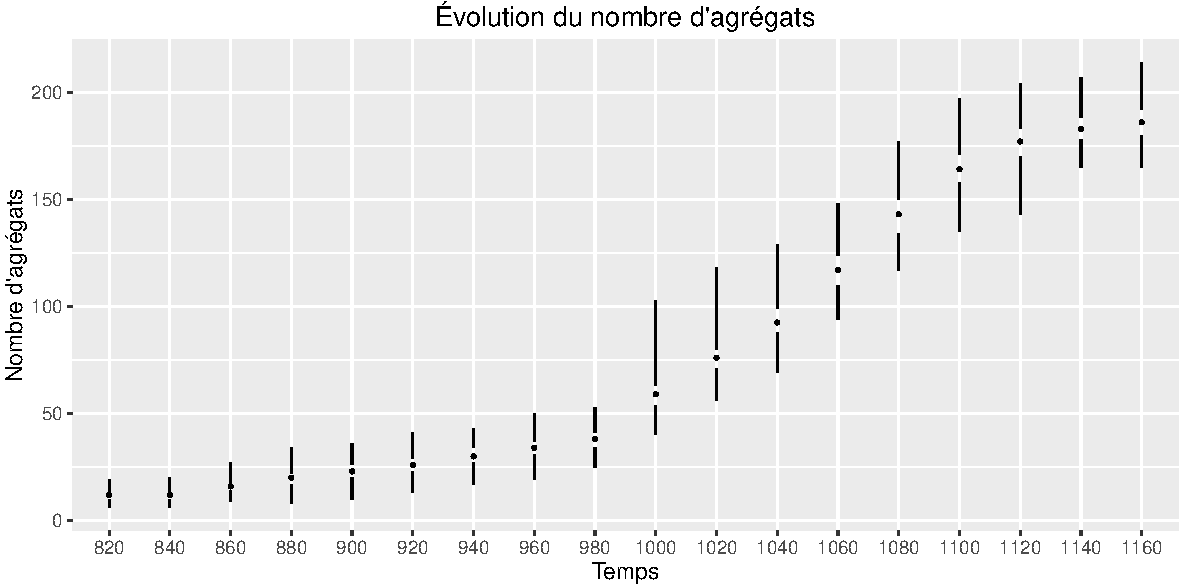
\includegraphics[width=\linewidth]{img/resultats/v0_nombre_agregats.pdf}
	\caption{Évolution du nombre d'agrégamouvementts.} 
	\label{fig:nombre-agregats-v0} 
\end{figure}

\todobox{
		Il y a un problème ici par rapport à ce qui a été mis dans le chapitre :
dans le chapitre TMD, on mentionne 83 agrégats en moyenne, alors que dans l'analyse de Base, il y en a 187...
}	

\paragraph{Nombre de pôles}\label{para:nb-poles}

Dans le modèle SimFeodal, les foyers paysans sont polarisés par des pôles d'attraction.
Pour une polarisation efficace, il est donc nécessaire que les pôles soient suffisamment nombreux, c'est-à-dire, \textit{a minima}, autant que d'agrégats attendus ($200$).
Contrairement aux agrégats, un nombre trop important de pôles ne constitue pas un problème :
en considérant que $20\%$ des foyers paysans doivent demeurer isolés en fin de simulation, il est vraisemblable qu'une partie des pôles, par exemple composés d'une église paroissiale, n'aient pas vocation à voir la constitution d'un agrégat autour d'eux.

Par ailleurs, afin de renforcer la polarisation par l'action de l'attraction différenciée -- selon le nombre de foyers paysans contenus dans chaque agrégat\footnote{\label{ftn:preferential-attachment}
	L'attraction qu'exercent les pôles contenant des agrégats de population est ainsi plus forte lorsque ces derniers sont constitués d'un nombre de foyers paysans important, et moindre quand ce nombre est faible.
Cela place ce mécanisme dans une logique proche de celle de l'attachement préférentiel identifié par \autocite{yule1925ii} et  \autocite{simon1955class}, cités par \autocite[93]{schmitt_modelisation_2014-1}) \label{ftn:attachement-preferentiel}
} --, il faut que le taux de pôles contenant un agrégat soit important, et surtout croissant au cours du temps :
comme dans l'empirie, cela est alors le marqueur que de petits pôles d'attractions, comme les églises paroissiales, parviennent à polariser suffisament de foyers paysans de leur voisinage pour aboutir à la création d'un petit agrégat, un village par exemple.

Pour un résultat satisfaisant, il faut donc que le nombre de pôles augmente régulièrement au cours de la durée de la simulation, et que le taux de pôles contenant un agrégat augmente lui aussi de manière continue.

\begin{mdframed}[backgroundcolor=gray!10,footnoteinside=false]
	L'évolution du nombre de pôles est assez représentative de l'empirie dans la version 0 de SimFeodal.
On aboutit ainsi sur $\textbf{190}$ pôles en moyenne en fin de simulation, ce qui est dans le bon ordre de grandeur, quoi qu'un peu trop faible.
Ce nombre est en croissance constante à partir de 940 (\cref{fig:nombre-poles-v0}).
Ce départ quelque peu tardif peut expliquer le relatif manque de pôles en fin de simulation.
	
	L'analyse de la constitution de ces pôles en matière d'agrégat est toutefois plus décevante :
la croissance n'est pas linéaire, stagnant entre 940 et 1000, puis à partir de 1040.
On constate ici un mauvais comportement du modèle par rapport à l'empirie :
il y a création de nombreux pôles, mais ceux-ci ne suffisent pas à polariser les foyers paysans.
On peut donc penser qu'il s'agit de nombreux pôles ruraux, par exemple composés d'une unique église paroissiale, ne suffisant dès lors pas à concentrer les foyers paysans alentours.
	
	Dans cette dimension, comme pour l'indicateur principal qu'en est le taux de foyers paysans dispersé, l'effet de la polarisation apparaît nettement trop faible.
\end{mdframed}


\begin{figure}[H]
	\captionsetup{width=\linewidth}
	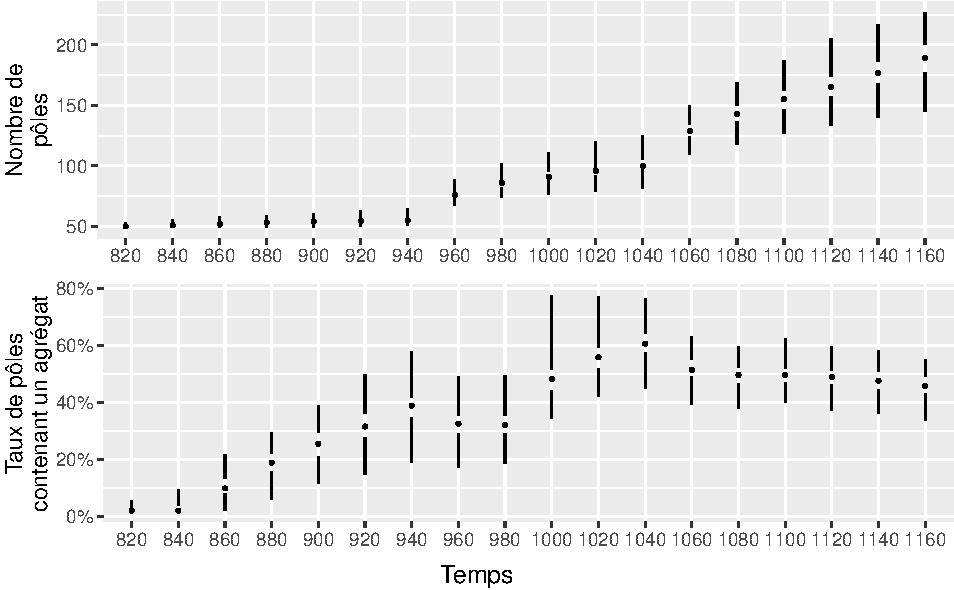
\includegraphics[width=\linewidth]{img/resultats/v0_nombre_poles.pdf}
	\caption{Évolution du nombre de pôles et du taux de pôles contenant un agrégat.} 
	\label{fig:nombre-poles-v0} 
\end{figure}

\paragraph{Dispersion des agrégats et pôles}\label{par:polarisation-dispersion}

Les indicateurs présentés ci-dessus avaient en commun d'être des indicateurs de sortie, générés automatiquement, et présentés sous forme d'agrégations des réplications.
Pour préciser l'analyse de la polarisation, il est toutefois nécessaire d'aborder une dimension qui n'est fondamentalement pas agrégeable dans les indicateurs de sortie :
l'espace du modèle.
Comme celui-ci est théorique et aléatoire, il n'y a aucun sens à agréger des entités différentes, par exemple des agrégats, sachant que ceux-ci occupent des localisation aléatoires et ne sont pas identifiables en tant que tels.

On ne peut cependant pas se passer d'une analyse spatiale de la répartition des pôles et agrégats afin de comprendre les dynamiques effectivement simulées par le modèle.
La distribution spatiale des agrégats et des pôles est en effet un facteur majeur de la polarisation :
s'ils sont très concentrés, les foyers paysans non présents alentours ne trouveront pas d'attracteurs à proximité, et ne seront de plus pas particulièrement affectés par l'augmentation des droits (banaux etc.) et des contraintes spatiales (proximité à une église, à un château etc.).
A l'inverse, des agrégats entièrement dispersés ne favoriseraient pas la structure spatiale hiérarchisée que l'on chercher à faire émerger.

Afin que le comportement du modèle soit satisfaisant, il faut donc que les pôles et agrégats occupent l'ensemble de l'espace du modèle, tout en présentant des zones de concentration relatives plus importantes.
Comme on ne peut agréger les représentations spatiales, il convient, pour cette analyse, de regarder individuellement un échantillon de configurations spatiales générées.

\begin{mdframed}[backgroundcolor=gray!10,footnoteinside=false]
	La lecture des cartes de répartition des agrégats et des pôles de deux réplications de la version 0 (\cref{fig:cartes-agregats-v0}) va, dans l'ensemble, dans le sens de l'empirie.
On peut ainsi remarquer que ces entités ont bien tendance, au cours du temps, à se disperser dans l'espace modélisé.
En fin de simulation, tout l'espace est occupé, et on remarque même que certaines zones voient une forte concentration en agrégats, reproduisant les faits stylisés connus.
La répartition spatiale des agrégats -- et des pôles -- est donc bonne, et ne semble pas opposer d'obstacle à la polarisation attendue du système de peuplement.
	
	Ce résultat peut cependant être nuancé par l'observation de la dynamique de cette dispersion :
on constate ainsi que la dispersion s'effectue rapidement (entre 800 et 940), et n'évolue plus vraiment après.
Ce phénomène est donc plus rapide dans cette version 0 du modèle que dans les connaissances empiriques de la région Touraine.
	
	On peut enfin remarquer, en préalable aux dynamiques de hiérarchisation du système que l'on s'apprête à étudier, que ces sorties illustrent un manque criant de hiérarchie quant à la composition des agrégats :
on ne remarque, visuellement, que peu de différence entre les agrégats, et surtout, cette hiérarchie semble faiblir entre 1040 et 1160 (les agrégats les plus importants ont vu leur nombre de foyers paysans diminuer).
\end{mdframed}

\begin{figure}[H]
	\captionsetup{width=\linewidth}
	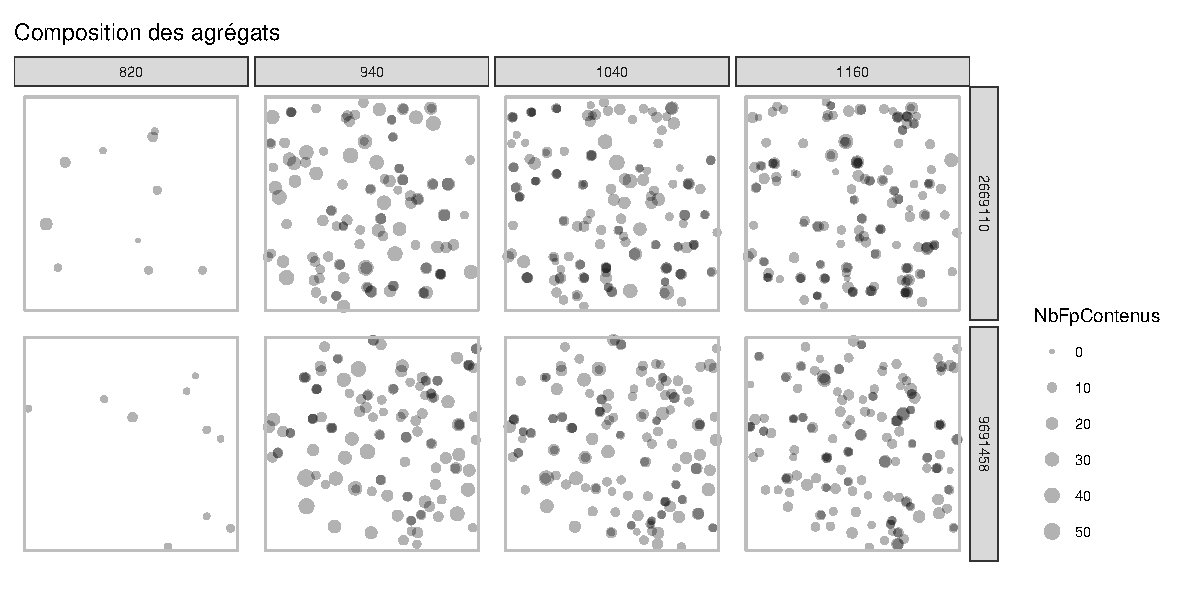
\includegraphics[width=\linewidth]{img/resultats/v0_cartes_agregats.pdf}
	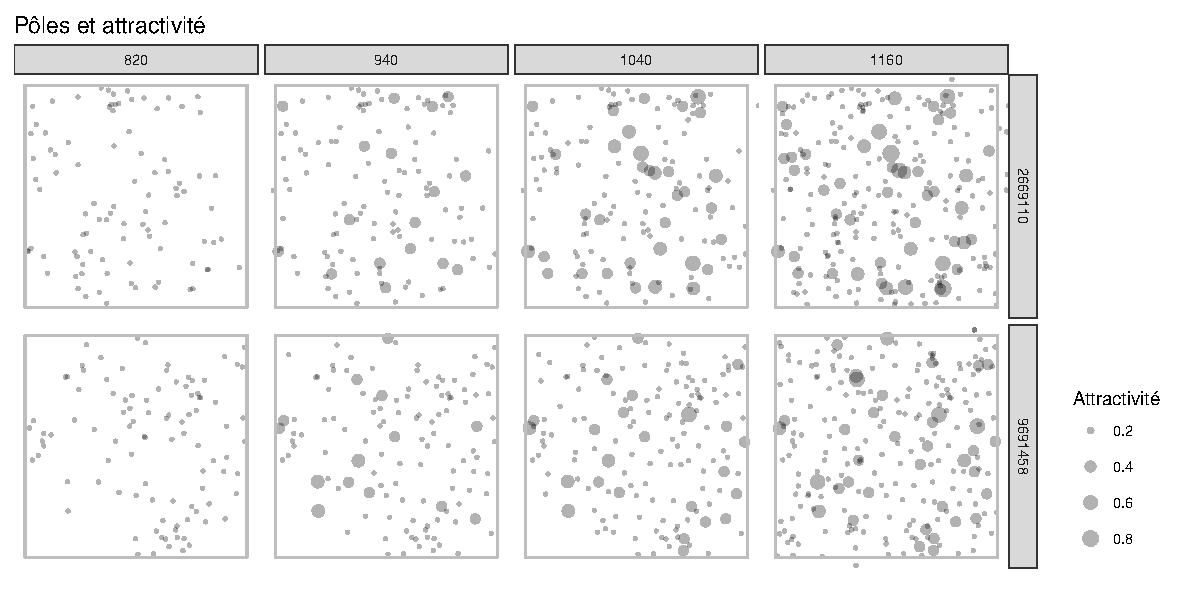
\includegraphics[width=\linewidth]{img/resultats/v0_cartes_poles.pdf}
	\caption{Évolution de la répartition spatiale des agrégats et pôles, pour deux réplications.} 
	\label{fig:cartes-agregats-v0} 
\end{figure}

\subsubsection{Évaluer la hiérarchisation du système de peuplement}

La seconde dimension de l'évaluation du modèle SimFeodal correspond à l'étude de la hiérarchisation du système de peuplement.
On déduit en effet des connaissances empiriques une forte hiérarchisation du système de peuplement sur la période, et plus généralement, des entités présentes.
On passe ainsi, en 800, d'un habitat dispersé dans lequel coexistent quelques agrégats de taille uniforme, à un habitat concentré dans des agrégats de taille très hétérogènes à la fin du XIIème siècle.
La distribution des tailles des agrégats est estimée par les connaissances expertes, toutes proportions gardées, comme assez proche des distributions observées aujourd'hui dans les systèmes de peuplement.
On souhaite ainsi que les agrégats modélisés suivent une distribution approchant la distribution log-normale.

Par extension, et là encore d'après les connaissances thématiques, l'ensemble des entités doit aussi suivre le même type de forme.
Par exemple, les pôles, tant en terme d'attractivité que de composition, doivent aussi montrer une hiérarchie du même ordre, ainsi que les seigneurs -- à travers leur puissance, au moins pour les petits seigneurs --, ou encore les paroisses, par le nombre de paroissiens qu'elles desservent.

Comme pour l'étude de la polarisation, on peut définir un indicateur principal de cette hiérarchisation du système de peuplement :
la forme de la distribution de la composition en foyers paysans des agrégats.

De la même manière que pour la polarisation, les indicateurs secondaires ont aussi pour but de préciser cet indicateur principal, et en particulier d'analyser les moteurs de cette hiérarchisation du peuplement.
On a en effet choisi d'observer plutôt la hiérarchisation des autres types d'entités -- pôles, seigneurs, paroisses --, pour vérifier qu'elles accompagnent et/ou entraînent bien la hiérarchisation des agrégats.
La hiérarchie des pôles, par exemple, a une influence directe sur l'attraction effectuée sur les foyers paysans (polarisation) et sur la hiérarchisation des agrégats :
par effet d'attraction différenciée (voir la note de bas de page \ref{ftn:attachement-preferentiel} \cpageref{ftn:attachement-preferentiel}), des agrégats plus importants se constituemouvementnt autour des pôles les plus importants.

Comme pour la polarisation, l'analyse de la capacité du modèle a reproduire la hiérarchisation du système de peuplement se fait donc en deux temps :
en premier lieu, on évalue cette capacité à l'aide de l'indicateur principal, puis on précise cette qualification et on essaie de l'expliquer à l'aide des indicateurs secondaires.


\paragraph{Hiérarchie des agrégats}

L'indicateur principal est un indicateur agrégé, correspondant à la forme de la distribution des agrégats mesurés par le nombre de foyers paysans qui les composent.
Cet indicateur est classique dans l'analyse des systèmes de peuplement, et il est courant de l'observer par le biais d'un indicateur agrégé simple, correspondant à la loi rang-taille.
On observe pour cela le modèle statistique, ou sa représentation graphique tout du moins, mettant en relation le logarithme de la taille des individus (le nombre de foyers paysans composant chaque agrégat ici) et le logarithme du rang de cet individu.
Comme pour toute régression linéaire, on peut alors quantifier l'ajustement du modèle grâce au coefficient de détermination ($R^2$), et spécifier la pente de la courbe, représentant le degré de hiérarchie, à travers le coefficient directeur ($a$ dans la formule $y = ax + b$).

Dans le cas de SimFeodal, le faible nombre d'agrégats ainsi que la variabilité de leurs tailles rend difficile cette analyse quantifiée, le coefficient directeur, par exemple, étant très sensible aux faibles effectifs.
On utilise toutefois la représentation graphique décrite comme un indicateur majeur de la hiérarchie des agrégats.

Du point de vue des connaissances empiriques, la courbe doit ainsi voir sa pente augmenter avec le temps, tout en devenant plus convexe, ce qui représente la \og longue traine\fg{} des petits agrégats, empiriquement observée dans toutes les distributions de systèmes de peuplement.

Avec une autre représentation graphique du même phénomène, en discrétisant les agrégats selon leur taille et en dénombrant le nombre d'agrégats de chaque classe, on peut aussi avoir une vision plus synthétique (car moins exhaustive) de la forme de la distribution.
On doit alors obtenir un nombre décroissant d'agrégats à mesure que la classe représente un nombre élevé de foyers paysans.

\todobox{
		Ça vaudrait peut-être le coup, pour chaque indicateur présenté sous forme graphique (évolution ou forme), de faire un graphique théorique (une sorte de courbe parfaite) de ce que l'on souhaite observer.
		}

\begin{mdframed}[backgroundcolor=gray!10,footnoteinside=false]
	La version 0 de SimFeodal présente une hiérarchisation des agrégats nettement trop faible.
La courbe rang-taille (\cref{fig:rt-agregats-v0}) est ainsi trop faiblement pentue, et présente une forme trop linéaire :
la convexité due à la longue traine n'est pas assez visible, en raison sans doute de trop faibles valeurs  en haut de la hiérarchie, qui ne \og tire\fg{} alors pas assez la distribution.
Ce résultat de simulation est d'autant plus perturbant que son évolution est éloignée de l'empirie :
on remarque en effet que la distribution se hiérarchise bien entre 800 et 1020, présentant à cette date une allure très satisfaisante.
Pourtant, après cette période, les agrégats voient leur hiérarchie diminuer nettement et les agrégats les plus peuplés diminuer en taille.
	
	On constate le même décrochage dans la discrétisation des agrégats (\cref{fig:compo-agregats-v0}), où on remarque de plus que la hiérarchie la plus proche de l'attendu, où la position des classes suivrait une ligne droite, semble se dessiner entre 940 et 1040.
En 1040, et plus encore en 1160, la proportion d'agrégats de taille moyenne et haute (de 30 à 100, et de plus de 100 foyers paysans) est trop faible, et pas assez hiérarchisée.
	
\end{mdframed}

\begin{figure}[H]
	\captionsetup{width=\linewidth}
	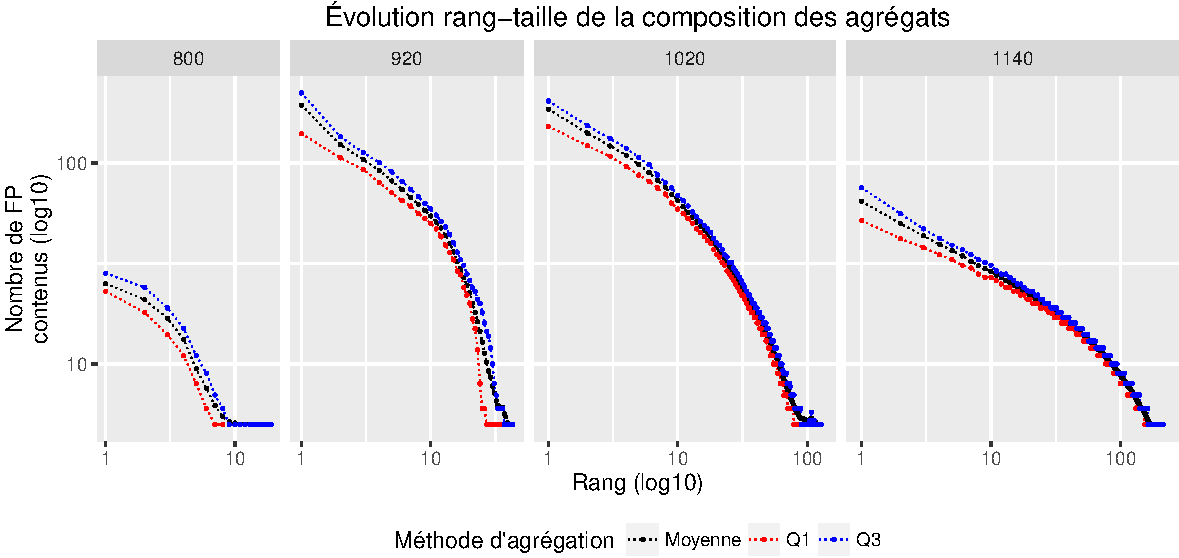
\includegraphics[width=.8\linewidth]{img/resultats/v0_rt_agregats.pdf}
	\caption{Évolution de la courbe rang-taille des agrégats.} 
	\label{fig:rt-agregats-v0} 
\end{figure}

\begin{figure}[H]
	\captionsetup{width=\linewidth}
	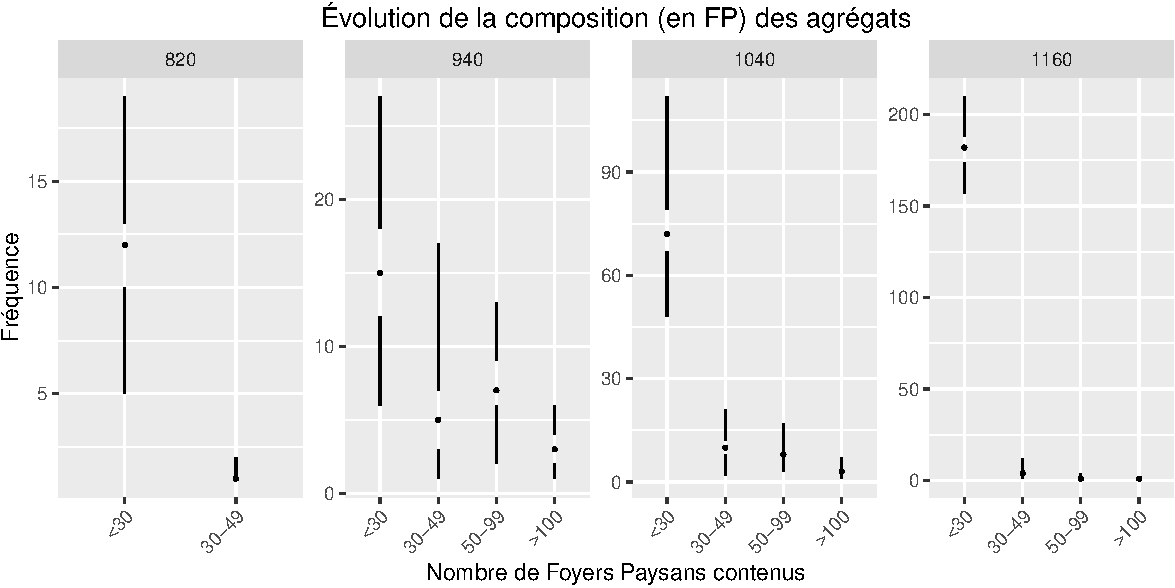
\includegraphics[width=.8\linewidth]{img/resultats/v0_compo_agregats.pdf}
	\caption{Évolution de la composition des agrégats.} 
	\label{fig:compo-agregats-v0} 
\end{figure}

\paragraph{Hiérarchie des pôles}

La hiérarchie des agrégats donne une bonne vision agrégée de la hiérarchisation du système de peuplement dans son ensemble.
Pour autant, afin d'appréhender la dynamique de cette dimension, il est là encore nécessaire d'observer le comportement des composantes qui provoquent cette hiérarchisation.
En effet, une forte hiérarchie des pôles entraînera une attractivité des foyers paysans très inégale \footnote{En raison des logiques d'attachement préférentiel, voir la note de bas de page \ref{ftn:preferential-attachment} page \pageref{ftn:preferential-attachment}.} De plus, comme indiqué plus haut, on cherche à obtenir une forte hiérarchi)e pour les différents types d'agents du modèle.
L'observation de la hiérarchie des pôles est donc importante pour évaluer le modèle SimFeodal.
Pour déterminer cette hiérarchie, on peut se fier à deux indicateurs complémentaires :
le nombre d'attracteurs composant chaque pôle et l'attractivité de ces derniers.
Ces indicateurs de sortie sont proches, mais apportent pourtant une vision légèrement différente :
étant donné que chaque attracteur influe différemment, selon son type, sur l'attractivité globale d'un pôle, l'information sur l'attractivité et sur la composition ne sont pas redondantes, bien que fortement corrélées.
On aurait pu présenter une information plus détaillée quant à cette composition, par exemple en différenciant le nombre de chacun des types d'attracteurs de chaque pôle, mais le nombre de combinaisons possible aurait rendu cette information confuse.

À partir des connaissances expertes qui guident l'évaluation de SimFeodal, on cherche à obtenir, pour ces deux indicateurs, une courbe d'allure similaire, c'est-à-dire une courbe décroissante, avec bien plus de pôles mineurs (faible attractivité ou nombre d'attracteurs) que de pôles plus importants.
On cherche de plus à ce que cette courbe présente une allure log-normale, et donc que la proportion de pôles décroisse fortement à mesure que leur importance augmente.


\begin{mdframed}[backgroundcolor=gray!10,footnoteinside=false]
	Dans l'ensemble, on peut remarquer sur les deux indicateurs de la \cref{fig:compo-poles-v0} que les pôles, dans cette version 0, sont très hiérarchisés.
La tendance \og évolutive va dans le bon sens :
depuis une quasi-uniformité en 820, des pôles plus importants apparaissent et semblent se renforcer au cours du temps.
On retrouve aussi, en observant les axes des ordonnées, la croissance du nombre de pôles identifiée plus haut (p. \pageref{para:nb-poles}) :
de nouveaux pôles apparaissent tout au long de la simulation, et restent majoritairement peu importants, quand les pôles ayant commencé à se renforcer tôt continuent dans cette tendance.
	
	En fin de période, les pôles sont très hiérarchisés, aussi bien en matière de composition que d'attractivité.
Ils le sont même plus que ce que les connaissances expertes laissent entendre :
au delà de $0.66$ en attractivité ou de $4$ attracteurs, on ne dénombre plus qu'un unique pôle de chaque importance, là où on attendrait que cette courbe continue plutôt à décroitre.
	De plus, ces courbes montrent la variation des réplications de la version 0.
	Dès lors, on peut considérer que ces pôles majeurs ne sont en fait qu'un unique pôle (le plus souvent) d'importance variable selon les réplications, mais dans tous les cas d'importance bien supérieure aux pôles qui arrivent juste après dans le classement.
Cette macrocéphalie ne correspond pas aux observations empiriques, d'autant que rappelons-le, la ville de Tours n'est pas modélisée dans SimFeodal.	
	

\end{mdframed}

\begin{figure}[H]
	\captionsetup{width=\linewidth}
	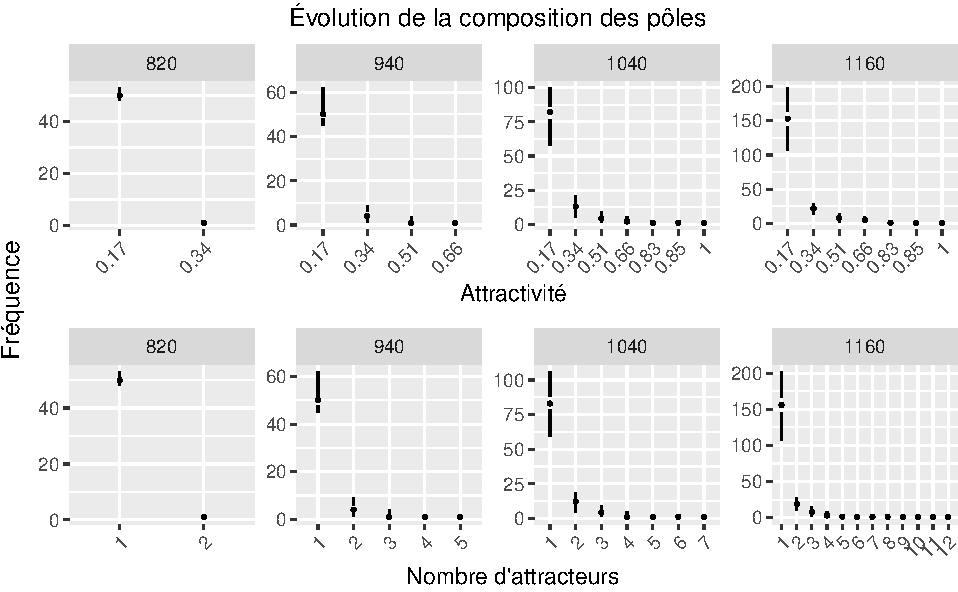
\includegraphics[width=\linewidth]{img/resultats/v0_compo_poles.pdf}
	\caption{Évolution de la composition et de l'attractivité des pôles\protect\footnotemark{}.} 
	\label{fig:compo-poles-v0}
\end{figure}
\footnotetext{\hl{Les figures ne sont pas en log-log (ou log-lin) et on ne voit donc pas vraiment le haut de la hiérarchie.
Peut-être faudrait-il changer ces axes, mais ça complexifiera la lecture pour les archéos/lecteurs non habitués aux axes log}}

\paragraph{Hiérarchie des paroisses}

A l'instar des pôles, on attend aussi des ressorts paroissiaux d'être hiérarchisés.
La période modélisée voit ainsi apparaître ces paroisses qui auront un rôle majeur dans la fixation du peuplement, et, pré-figurant le maillage communal, ont un double rôle de desserte efficace\footnote{C'est-à-dire desservir de manière optimale le plus gros de la population.} et équitable\footnote{C'est-à-dire faire en sorte que même les populations les plus isolées aient un accès aussi rapide que possible à une église paroissiale.}.
En effet, avec la volonté d'encadrement et de prélèvement de l'Église sur la population, de nouvelles paroisses apparaissent pour desservir au mieux leurs potentielles ouailles.
Une structure double en résulte :
dans les zones les moins denses, le maillage est régulier mais lâche, de manière à minimiser le nombre d'églises paroissiales tout en s'assurant que chacun puisse y accéder dans un temps raisonnable\footnote{Cette distance-temps évolue au cours du temps, en fonction de l'accroissement de la fréquence de l'obligation de fréquentation des églises paroissiales.}.
Il y a donc un certain nombre d'églises paroissiales desservant peu de paroissiens.
Au contraire, dans les zones les plus denses, et en particulier au sein des petites villes naissantes, l'objectif est d'être au plus près des résidents tout en garantissant à chacun de pouvoir assister aux différents offices :
il y donc une croissance du nombre d'églises paroissiales proches les unes des autres, visant à accompagner un encadrement maximum de la population, ainsi, avec une logique concurrentielle de ce clergé féodal, qu'à capter l'importante source de revenus qu'assure la collecte de la dîme.
Cette logique concurrentielle doit aussi permettre de restreindre le nombre de foyers paysans desservis par une unique paroisse.

On s'attend donc à avoir une courbe hiérarchisée dans la lignée d'une courbe log-normale, mais avec toutefois un double seuil minimal (l'effet de \og longue traîne\fg{}), autour des paroisses \og rurales\fg{} peu peuplées (moins de 10 foyers paysans désservis) et des paroisses du bas de la hiérarchie classique, peuplées de 10 à 40 foyers paysans\footnote{D'après les valeurs des paramètres \texttt{nb\_min\_paroissiens} et \texttt{nb\_max\_paroissiens}}).

\todobox{ici, impérativement, il faudra mettre un graphique schématique de ce qu'on attend.}

\begin{mdframed}[backgroundcolor=gray!10,footnoteinside=false]
	En fin de simulation de cette version 0, la hiérarchie des paroisses est plutôt satisfaisante.
On y retrouve en effet une forte hiérarchie, peut-être même légèrement trop importante.
Il ne devrait ainsi par y avoir de paroisse composée de plus de $100$ foyers paysans en fin de simulation, et la courbe présente une pente trop importante (celles de 940 ou 1040 sont ainsi plus conformes aux attentes).
	Pour autant, on remarque bien un effet de hiérarchisation au cours du temps, ainsi qu'un accroissement du nombre de petites paroisses, montrant que la dynamique, bien que non ajustée, s'inscrit bien dans la dynamique observée empiriquement.
	(\cref{fig:compo-paroisses-v0})
\end{mdframed}

\begin{figure}[H]
	\captionsetup{width=\linewidth}
	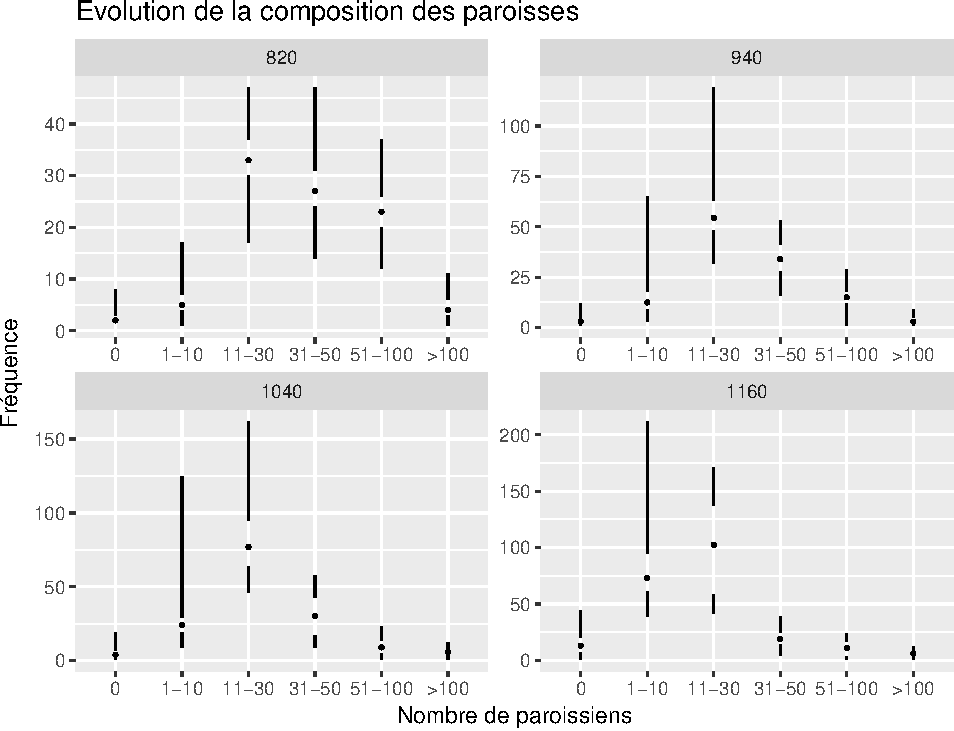
\includegraphics[width=\linewidth]{img/resultats/v0_compo_paroisses.pdf}
	\caption{Évolution de la composition des paroisses.} 
	\label{fig:compo-paroisses-v0} 
\end{figure}


\subsubsection{Évaluer la fixation et la dissémination du peuplement}


La dernière dimension étudiée par SimFeodal est moins définie que les précédentes.
On y observe ainsi la fixation du système de peuplement au sein du maillage naissant que constituent les paroisses.
Cette notion de fixation pose problème par rapport à l'ensemble des indicateurs de sortie déployés jusqu'ici.
En effet, SimFeodal est un modèle fondé sur un temps discret :
on y observe, à chaque itération, le résultat des processus modélisés.
On peut y observer une fixation d'un pas de temps par rapport à l'autre, par exemple en constatant qu'un agrégat constitué en 820 semble être toujours présent en 840.
On peut de plus considérer que cet agrégat présente les mêmes caractéristiques au deux dates, en matière de localisation et de population.
L'agrégat est donc stable dans le temps.
L'échelle d'analyse mobilisée dans les indicateurs précédents -- au niveau agrégé des agrégats, voir du système d'agrégats -- pourrait donc s'appliquer ici aussi.
Pourtant, quand on parle de fixation des foyers paysans, ce qui est observé empiriquement, il n'est pas question d'agrégats, mais des entités les composant, c'est-à-dire les foyers paysans.
Ceux-ci ne sont pas observés directement quand on remarque que les agrégats semblent stable :
on approche là à la différence entre un état stable et un état stationnaire.
La relative stationnarité des agrégats dans le temps n'est ainsi pas garante de stabilité de leurs composantes :
deux foyers paysans oscillant d'un agrégat à un autre, dans un mouvement opposé, produiraient ainsi une stationnarité de ces agrégats, mais, en se déplaçant, ils ne satisferaient pas au critère de fixation.
Il y a donc un problème de changement d'échelle pour observer la fixation des foyers paysans :
il n'est plus possible de raisonner à l'échelle des agrégats, et il faut se concentrer sur celle des foyers paysans.

Cette échelle pose un autre problème :
les foyers paysans sont très nombreux ($4000$ dans la version 0) et se déplacent.
Ils se déplacent de plus selon des modalités très différentes (\hl{Faire ref aux mécanismes de déplacement du chapitre 2}), rendant complexe la caractérisation des mouvements de chacun et plus encore celle d'une agrégation de ces catégories.

Pour ces raisons, la production d'indicateurs synthétiques spatiaux -- une ou plusieurs cartes -- ne suffirait pas à communiquer une information intelligible sur l'éventuelle fixation des foyers paysans.
Il nous faut donc faire appel à des \og proxys\fg{}, non spatiaux, pour évaluer la fixation des foyers paysans.

A cet effet, on a retenu des indicateurs relatifs aux déplacements des foyers paysans et à leur raison :
combien de foyers paysans se déplacent à chaque pas de temps (moins il y a de déplacement, plus la fixation est importante) ? Quelles sont les modalités de ces déplacements (un déplacement entre deux agrégats lointains n'a pas les mêmes conséquences en terme de stabilité qu'un déplacement minime au sein d'un même agrégat) ? Ou encore, comment évolue la satisfaction des foyers paysans, et avec celle-ci, la probabilité de se déplacer ?

Ces indicateurs permettent d'évaluer la capacité du modèle à reproduire la fixation des foyers paysans.
Pour autant, la contrainte est ici double :
on recherche une fixation, mais celle-ci est, empiriquement, supposée se dérouler et se voir renforcer par la mise en place du maillage paroissiale qui doit servir de support à la nouvelle configuration spatiale émergente.

On s'appuiera donc aussi sur des indicateurs relatifs à cet espace support constitué par les paroisses :
leur nombre, leur dispersion dans l'espace et l'efficacité de la desserte qu'elles assurent.

\paragraph{Déplacement des foyers paysans}

Le déplacement des foyers paysans est l'élément moteur de SimFeodal :
c'est par le déplacement individuel de chacun des foyers paysans que la configuration spatiale évolue.
Les déplacements affectent donc chacune des dimensions d'analyse -- polarisation, hiérarchisation et fixation --, mais c'est au sein de cette dernière qu'il est le plus intéressant de les observer.
Il est en effet attendu que de nombreux déplacement surviennent, afin que le système de peuplement puisse se structurer, mais pour autant, il est aussi nécessaire que ces déplacements tendent à diminuer au cours du temps, une fois le système en voie de stabilisation.

On pourrait donc attendre que les déplacements suivent une courbe négative (linéaire ou non) tendant vers 0, impliquant une absence de déplacements en fin de période.
Pour autant, le mécanisme de déplacement est sans doute l'un des plus complexes du modèle, et on ne peut l'appréhender aussi simplement.

En premier lieu, les mécanismes de SimFeodal différencient deux types de déplacements (\hl{Faire ref à chap2}) :
les déplacements locaux (dans un rayon de $2500$m dans la version 0) et les déplacements lointains.

\begin{itemize}
	\item Les déplacements locaux visent à faire s'agréger des foyers paysans dispersés autour de pôles présents à proximités.
	Ce mécanisme peut être présent sur toute la durée de la simulation, sur un effectif faible.
	En effet, cet effet d'agrégation locale permet \og d'optimiser\fg{} la répartition spatiale des agrégats, en renforçant leur hiérarchie et en faisant fusionner des agrégats qui seraient très proches les uns des autres.
	Pour autant, dans un objectif de fixation du peuplement, il est nécessaire de veiller à ce que les foyers paysans ne soient pas amenés à se déplacer localement de manière continuelle, par exemple en faisant des allers-retours entre des pôles ou agrégats spatialement proches.
	
	\item Les déplacements lointains servent un autre rôle :
un foyer paysan qui ne serait pas en mesure d'augmenter sa satisfaction localement -- faute de pôles suffisamment attractifs dans le voisinage -- a une probabilité de se déplacer vers un agrégat situé n'importe où dans l'espace modélisé.
	Le modèle est très sensible à ce mécanisme qui agit comme une perturbation forte dans la structure spatiale du peuplement.
	Ce mécanisme \og de dernier recours\fg{} ne doit être employé que rarement, en cas de situations où des foyers paysans seraient trop isolés pour pouvoir s'agréger localement.
	C'est notamment le cas pour les foyers paysans nouveaux arrivants, via le mécanisme de renouvellement (\hl{ref dans chap 2}), qui peuvent se voir localisés n'importe où dans l'espace du modèle.
\end{itemize}

Pour ajouter à la complexité du mécanisme, et donc de l'évaluation de cet indicateur qu'est le nombre de déplacements au cours du temps, rappelons que différentes contraintes temporelles viennent bouleverser, à dessein, le comportement des foyers paysans.
En particulier, entre 950 et 1050, les modalités d'évaluation de la satisfaction deviennent plus strictes (\hl{Voir dans chap2, frise}).
Cela engendre nécessairement une plus forte propension des foyers à se déplacer.

Si les connaissances empiriques d'un tel niveau de finesse ne sont pas disponibles, on peut tout de même avoir des attentes quant au comportement attendu du modèle.
Au regard des éléments décrits plus haut, on peut ainsi chercher à ce que l'évolution des déplacements suive plusieurs rythmes au cours du temps :
\begin{enumerate}
	\item Dans une première phase, du début de la simulation jusqu'aux perturbations débutant en 950 :
quelques déplacements lointains marginaux ($\approx 5$\% à $10$\%), stables au cours du temps ; et de plus nombreux (au moins $\approx 30$\%) déplacements locaux menant à la constitution de petits agrégats locaux.
		Les déplacements locaux doivent diminuer au cours du temps, une fois les agrégats constitués.
	\item Pendant la deuxième phase, entre 950 et 1050, les nombreuses perturbations devraient voir une nette augmentation des déplacements locaux, et dans une moindre mesure lointains, prémices à la constitution d'agrégats plus hiérarchisés.
	\item Après ces perturbations, on devrait retrouver le niveau de déplacement de la seconde période, et là aussi, tendre vers une diminution des déplacements locaux, le système se stabilisant à l'approche de la fin de la période.
\end{enumerate}

Tout au long de cette période, on cherche de plus à ce que les foyers paysans soient polarisés, c'est-à-dire ici, qu'ils se regroupent dans des agrégats de population.
Parmi les modalités de déplacement, un autre indicateur utile est ainsi l'observation des provenances et destinations des foyers paysans qui se déplacent :
plus les foyers paysans originellement dispersés auront tendance à rejoindre des agrégats, plus la simulation sera satisfaisante au regard des hypothèses empiriquement émises.


\begin{mdframed}[backgroundcolor=gray!10,footnoteinside=false]
Dans cette version 0 de SimFeodal, il apparaît en premier lieu que les déplacements sont trop peu nombreux (\cref{fig:nb-deplacements-v0}).
Les déplacements lointains sont à peu près dans les proportions attendues, mais les déplacements locaux sont trop peu nombreux.
Surtout, les trois phases attendues ne se retrouvent pas sur ces sorties.
On y remarque bien l'impact des perturbations, mais celles-ci ne font qu'augmenter la part de déplacements, laquelle reste stable avant et après ces perturbations.
La version 0 de SimFeodal n'est donc pas satisfaisante en termes de stabilisation et de fixation des foyers paysans.
	
	L'observation des modalités de déplacement (\cref{fig:type-deplacements-v0}) montre certes une part croissante de déplacements \og Isolé -> Agrégé\fg{}, mais dans des proportions là aussi trop faibles passé le tout début de la simulation.
\end{mdframed}


\begin{figure}[H]
	\captionsetup{width=\linewidth}
	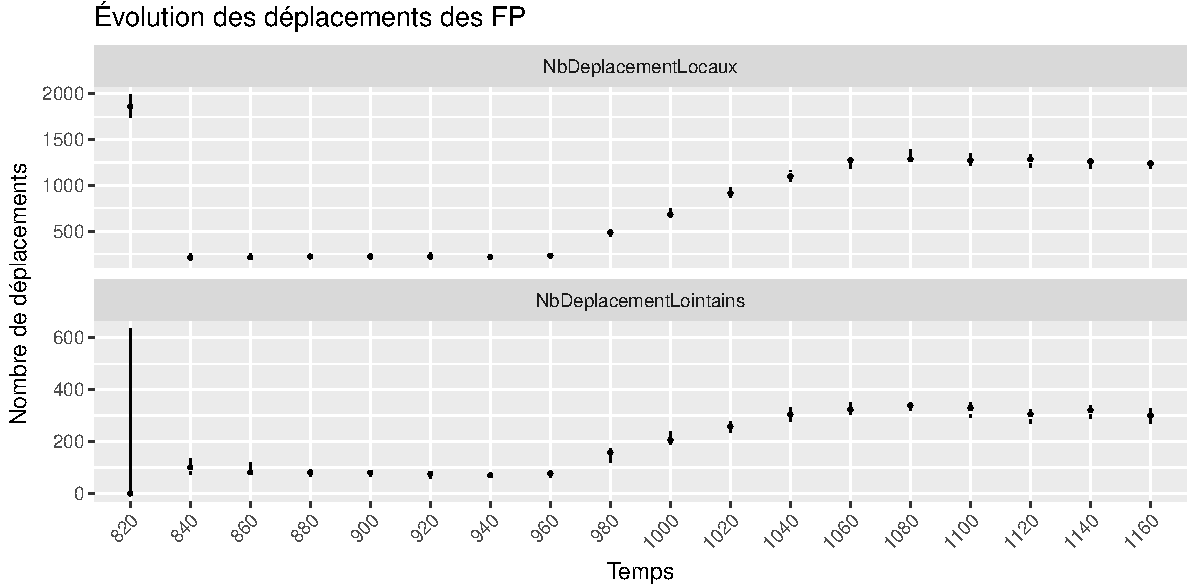
\includegraphics[width=\linewidth]{img/resultats/v0_nombre_deplacements.pdf}
	\caption{Évolution du nombre de déplacement des foyers paysans.\\
	\todobox{Mettre le graphique en relatif}} 
	\label{fig:nb-deplacements-v0} 
\end{figure}



\begin{figure}[H]
	\captionsetup{width=\linewidth}
	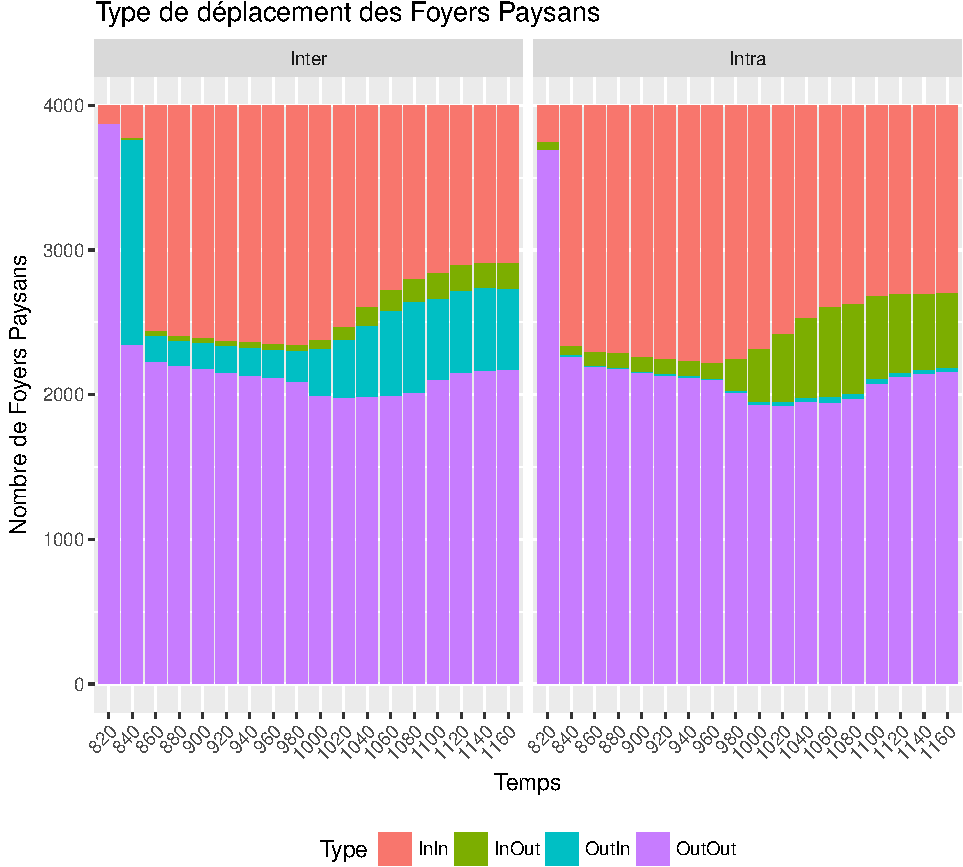
\includegraphics[width=\linewidth]{img/resultats/v0_types_deplacements.pdf}
	\caption{Évolution des types de déplacement des foyers paysans.\\
		Inter : Déplacement depuis le pas de temps précédent vs Intra :
déplacement au sein d'un même pas de temps.
		\todobox{Ne garder que l'inter et mettre le graphique en relatif}\\
%	- InIn : Le FP était dans un agrégat au pas de temps précédent, et est dans un agrégat à ce tour (quel qu'il  soit, ça peut être le même ou un autre).\\
%	- InOut : Le FP était dans un agrégat au pas de temps précédent, et est isolé à ce tour\\
%	- OutIn : Le FP était isolé, et est maintenant dans un agrégat\\
%	- OutOut : Le FP était isolé, et l'est toujours\\
%On constate donc que les déplacements au sein d'un tour tendent à isoler les FP, grosso modo dans le même temps et les mêmes proportions que la stabilisation du taux de FP isolés.	
} 
	\label{fig:type-deplacements-v0} 
\end{figure}



\paragraph{Satisfaction des FP}

Impact directement la fixation :
quand FP trop mécontents, ne se fixent jamais à un endroit et l'apparente stabilité des agrégats n'est due qu'à un effet pendulaire qui se compense à peu près.

\begin{mdframed}[backgroundcolor=gray!10,footnoteinside=false]
	(\cref{fig:satisfaction-fp-v0}).
\end{mdframed}

\begin{figure}[H]
	\captionsetup{width=\linewidth}
	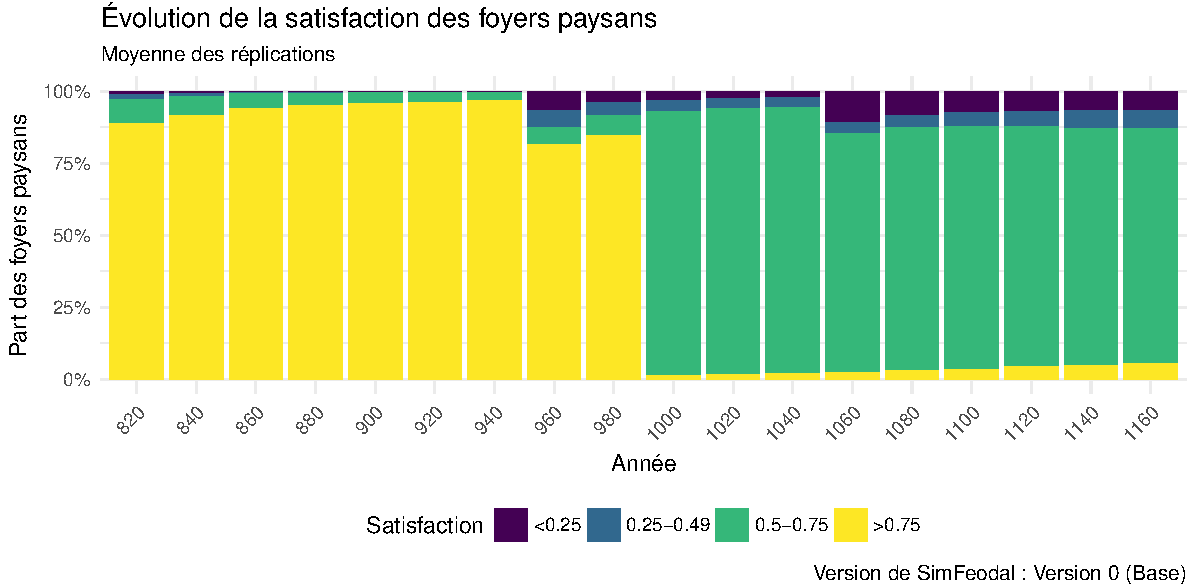
\includegraphics[width=\linewidth]{img/resultats/v0_satisfaction_fp.pdf}
	\caption{Satisfaction des foyers paysans} 
	\label{fig:satisfaction-fp-v0} 
\end{figure}


\paragraph{Nombre de paroisses}

\begin{mdframed}[backgroundcolor=gray!10,footnoteinside=false]
	(\cref{fig:nb-paroisses-v0} ).
\end{mdframed}

\begin{figure}[H]
	\captionsetup{width=\linewidth}
	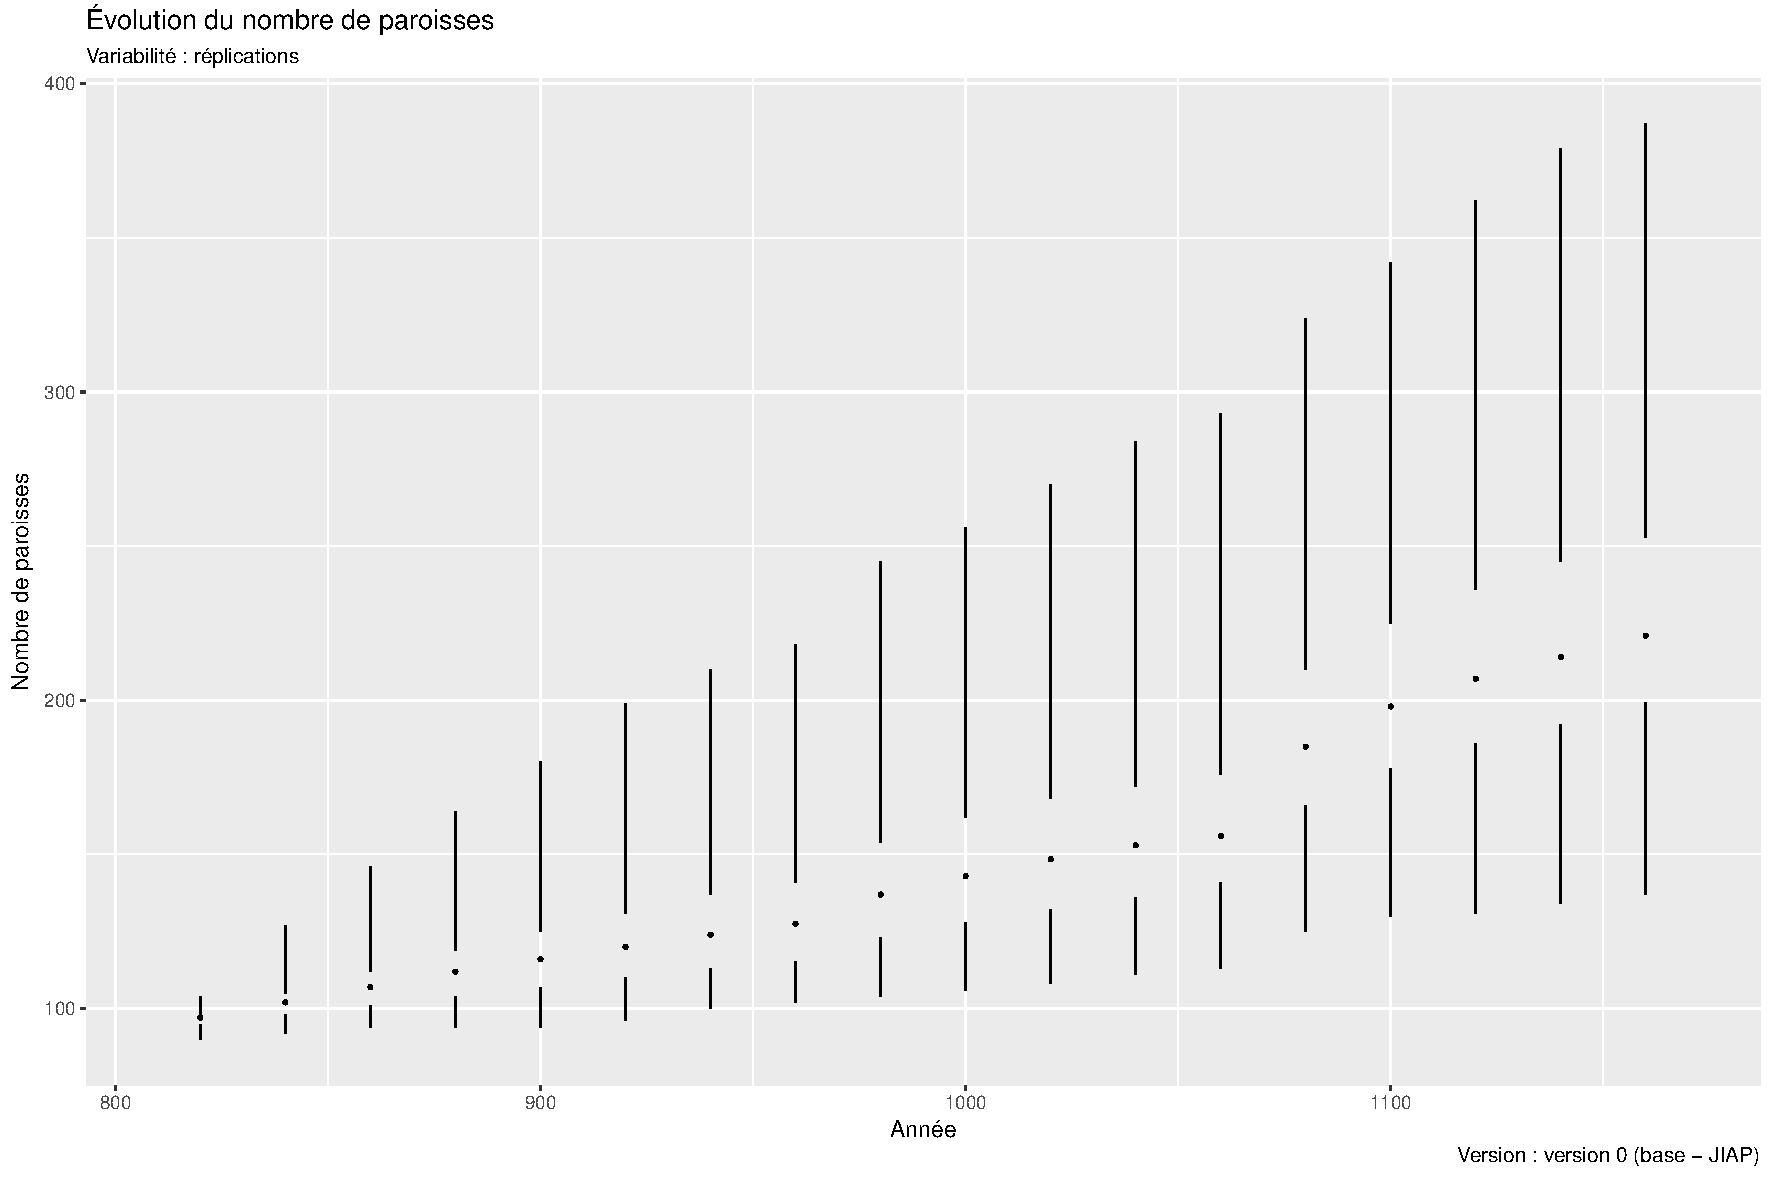
\includegraphics[width=\linewidth]{img/resultats/v0_nombre_paroisses.pdf}
	\caption{Évolution du nombre de paroisses} 
	\label{fig:nb-paroisses-v0} 
\end{figure}


\paragraph{Dispersion des paroisses}
Voir aussi la dispersion des agrégats et pôles (\autoref{par:polarisation-dispersion}, p. \pageref{par:polarisation-dispersion}) 

\begin{mdframed}[backgroundcolor=gray!10,footnoteinside=false]
	(\cref{fig:densite-paroisses-v0;fig:couverture-paroisses-v0} ).
\end{mdframed}


\begin{figure}[H]
	\captionsetup{width=\linewidth}
	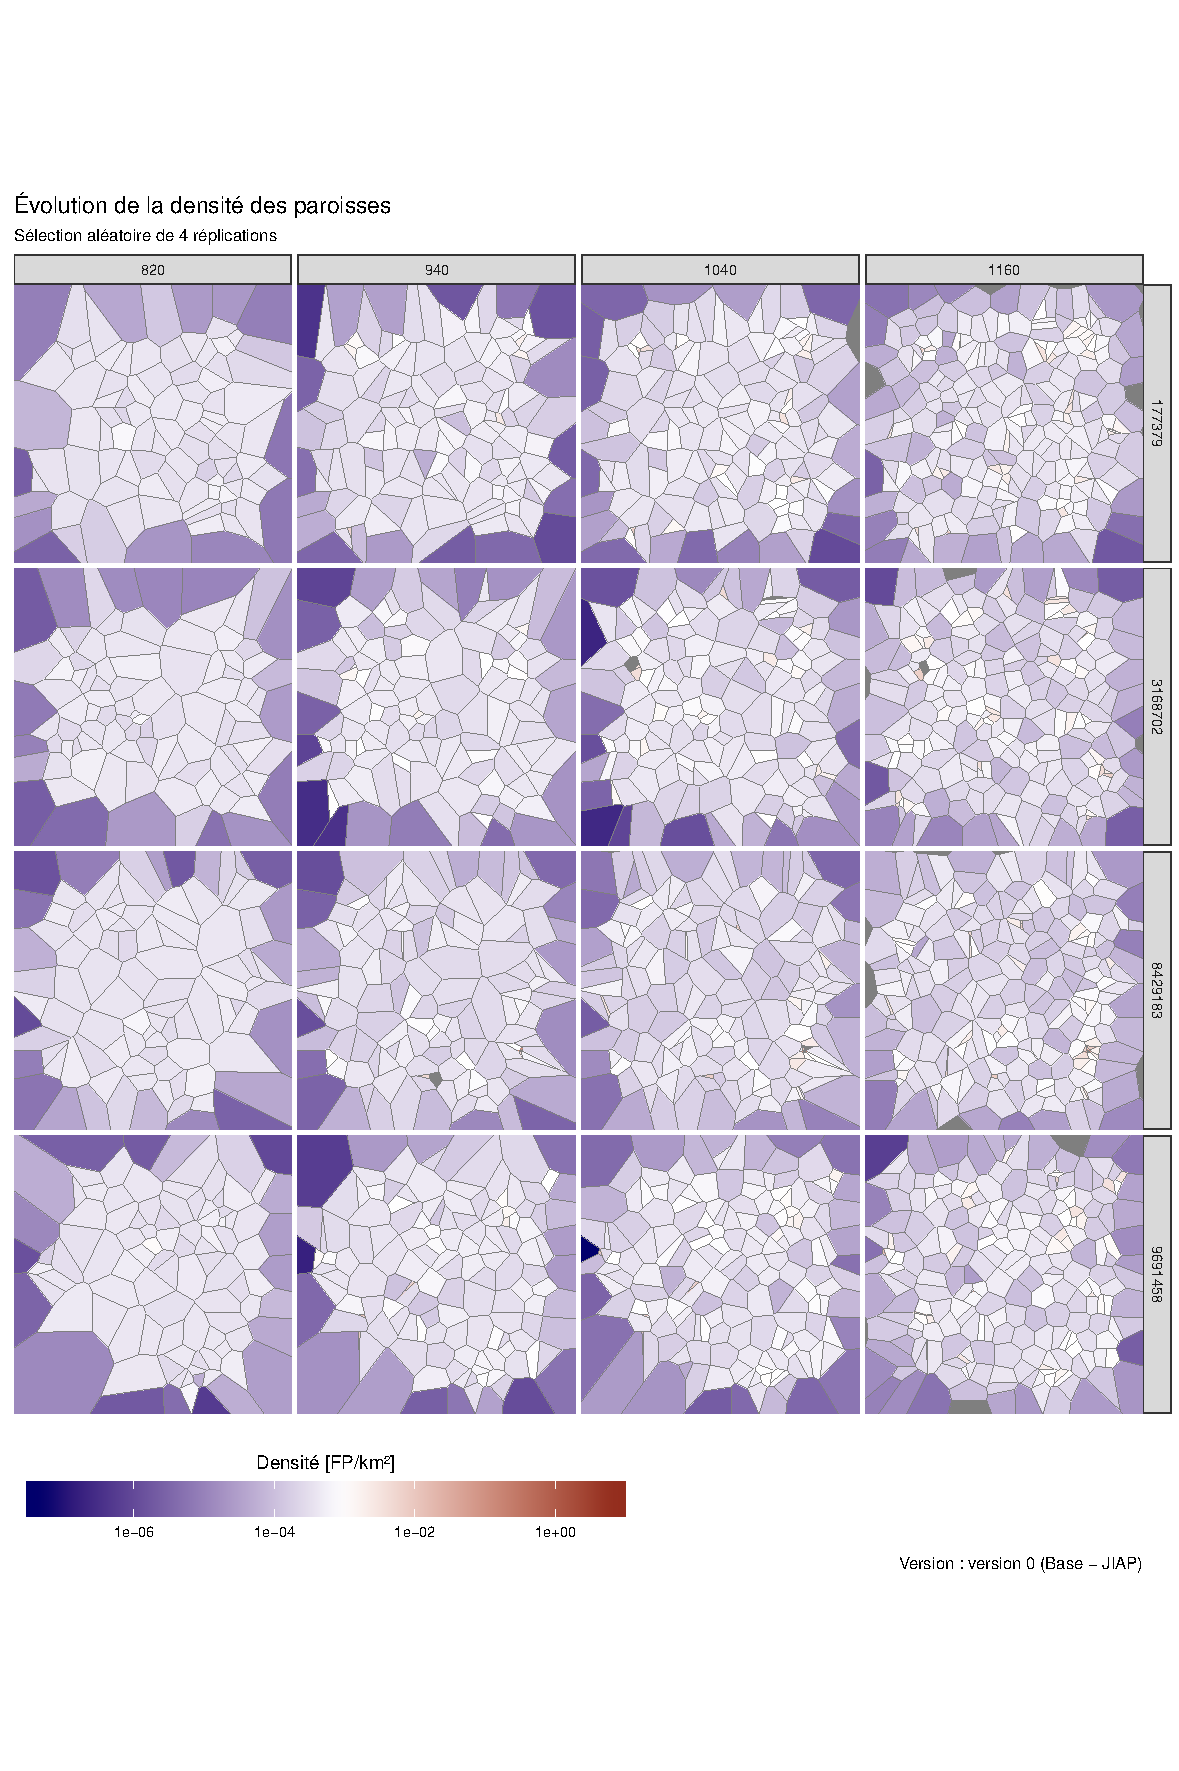
\includegraphics[width=\linewidth]{img/resultats/v0_paroisses_densite.pdf}
	\caption{Densité des paroisses} 
	\label{fig:densite-paroisses-v0} 
\end{figure}



\begin{figure}[H]
	\captionsetup{width=\linewidth}
	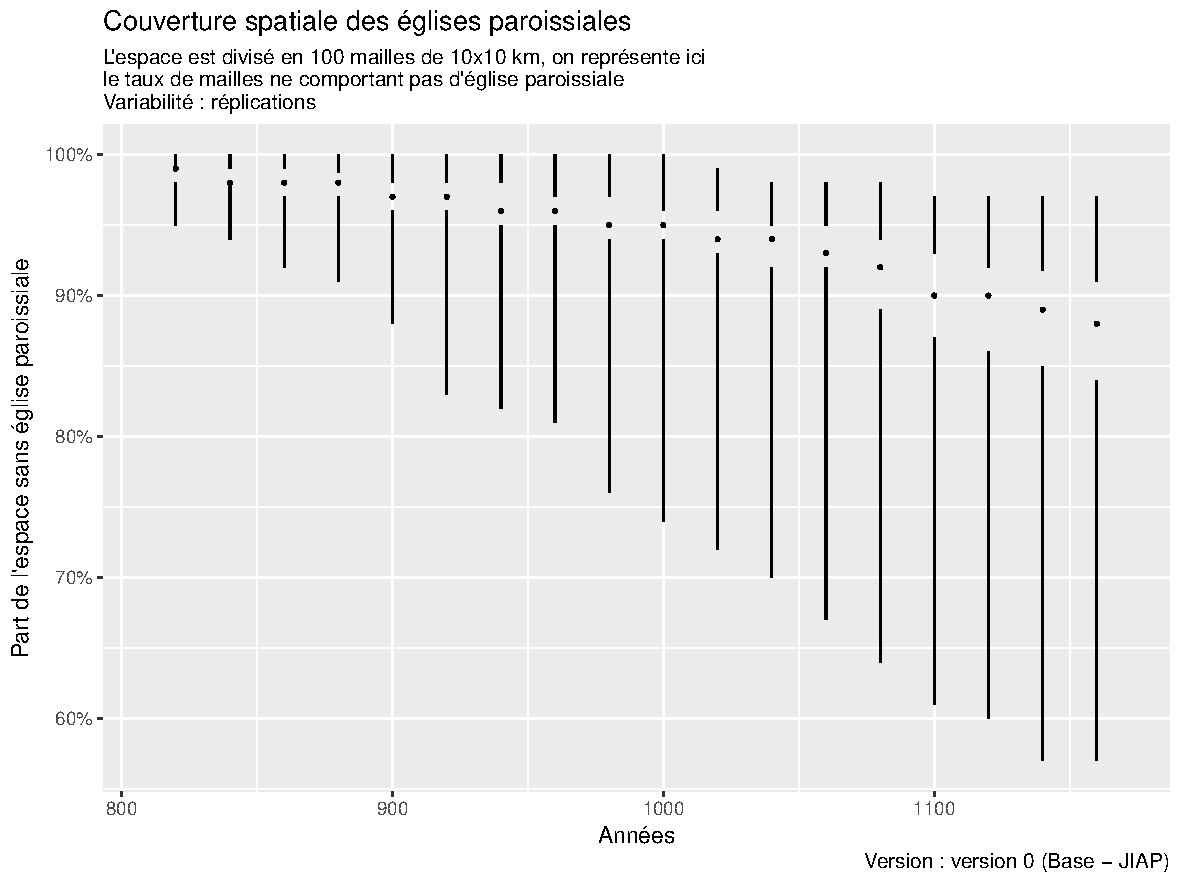
\includegraphics[width=\linewidth]{img/resultats/v0_paroisses_occupation.pdf}
	\caption{Évolution de la couverture du territoire par les églises paroissiales} 
	\label{fig:couverture-paroisses-v0} 
\end{figure}
Carte + indice type nb mailles occupées

\paragraph{Efficacité de la desserte}

\begin{mdframed}[backgroundcolor=gray!10,footnoteinside=false]
	???
\end{mdframed}

Distance des 10\% de FP les plus éloignés à une église paroissiale ?


%	\section[Évaluer SimFeodal]{Évaluer le modèle SimFeodal}
%	\subsection{Indices et indicateurs}
%	\subsection{Organiser et hiérarchiser les indicateurs}
%	\subsection{Les indicateurs et dimensions de SimFeodal}
	
	
%	\clearpage
\section{Paramétrage de SimFeodal}
	
\subsection{Avant propos sur le paramétrage d'un modèle complexe}
	
	\todobox{
	A changer : le chap 2 présentera la version 0 (Base) du modèle, et on vient donc ici montrer comment on a répondu aux limites identifiées à la fin du chapitre, cf. les conclusions/résultats du chapitre TransMonDyn.
	}
\medbreak
	
	\todobox{
	Pour introduire le schéma des étapes, rappeler ici que les paramètres et mécanismes d'un modèle complexe sont en interaction, ce qui produit des effets non linéaires.\\
	Principe des vases communicants !\\
	Mentionner aussi la logique des attracteurs étranges de Lorenz comme paroxysme de cette complexité : ici, moins de variation, mais des répercussions importantes tout de même qu'il faut donc \og corriger\fg{} par de nombreuses itérations de modifications.
	}

Le tableau suivant (\cref{table:etapes-construction}) se veut être un point de repère autant qu'une table des matières synthétique pour la compréhension des étapes qui suivent. Si la description de chacune de celles-ci revêt une forme assez factuelle et systématique, nous pensons toutefois que l'explicitation de chacune de ces étapes permet de saisir la démarche proposée ainsi que l'intérêt de celle-ci.

Notons que l'étape 0 ici présentée correspond à une première version \og exploitable\fg{} du modèle, c'est-à-dire contenant \textit{a minima} l'ensemble des agents et mécanismes identifiés dans un premier temps par l'équipe de modélisation \autocite{tannier_ontologie_2014-2}. Nous ne détaillerons pas ici les différentes phases de construction précédentes. Nous reviendrons toutefois sur plusieurs d'entre elles, en guise d'exemples illustratifs, dans les chapitres 6 et 7 \hl{(Partie 3)}.

\subsubsection{De manière générale}
	
\subsection{Les étapes du paramètrage de SimFeodal}
	
Comme préconisé ci-dessus, le modèle SimFeodal a été paramétré tout au long de sa construction. Dans cette partie, nous reviendrons en détail sur chacune des étapes de ce paramétrage, en retraçant les choix et questionnements qui ont orienté ces modifications du modèle. L'énumération est en ordre chronologique, et l'on a essayé d'organiser ces étapes en grands blocs-type de paramétrisation. Pour autant, le paramétrage et la construction d'un modèle, et du notre en particulier, sont un travail constant d'allers-retours entre l'identification et la résolution de problèmes. La structure réelle de développement, que l'on peut retrouver dans l'historique des modifications du modèle (les \og \textit{commits}\fg{}), ne correspond donc pas exactement à la chronologie organisée qui suit.
	
	
\pagebreak
\begin{footnotesize}
	\begin{longtable}{ m{.05\textwidth} m{.08\textwidth}  m{.12\textwidth}  m{.65\textwidth}  m{.10\textwidth}  }
		\caption{Tableau récapitulatif des étapes de construction du modèle. Conception : C. Tannier (\fixref{Tannier 2017, HDR}) et R. Cura, 2017}\\
		\label{table:etapes-construction}\\
		Étape & Version & Type      & Modifications                                                 & Section                                                                                   \\
		\endfirsthead
		Étape & Version & Type      & Modifications                                                 & Section                                                                                   \\
		\endhead			
		\hline
		0      & Base    & Création & Création du modèle. \fixref{Cf. tableau 14 de Tannier 2017} & Chap 2\footnote{On s'appuie sur cette version \og Base\fg{} dans le \fixref{chapitre 2}.} \\
		\hline
		1 & Base2 & paramétrage & \colorbox{yellow}{Hiérarchisation} des valeurs d'attraction des attracteurs. \newline
		Modification des critères de création de nouvelles paroisses. \newline
		Réduction de la distance maximale de déplacement local. \newline
		Assouplissement des règles de promotion d'un château en gros château. & Chap3-x.y\\
		\hline
		2 & Base2 compo5 2bis & modélisation et paramétrage & Assouplissement des règles de création d'une paroisse.\newline
		Réduction de la distance maximale de déplacement local. \newline
		Modification des règles de calcul de la probabilité de construire un château.\newline
		Modification du calcul de la satisfaction matérielle des foyers paysans. & Chap3-x.y\\
		\hline
		3 & Base2 compo5 2quat & modélisation et paramétrage & \colorbox{yellow}{Hiérarchisation} des valeurs d'attraction des attracteurs. \newline
		Facilitation de la construction de châteaux. \newline
		Rationnalisation du déplacement des foyers paysans. \newline
		Ajout d'un nouveau type d'attracteur, les communautés. & Chap3-x.y\\
		\hline
		4 & Base3 2 & modélisation et paramétrage & \colorbox{yellow}{Hiérarchisation} des valeurs d'attraction des attracteurs. \newline
		Modification des critères de création de nouvelles paroisses. \newline
		Augmentation de la distance maximale de déplacement local. \newline
		Modification de la procédure d'identification des agrégats et des pôles. & Chap3-x.y\\
		\hline
		5 & Base4 1 & modélisation et paramétrage & 
		Modification de la répartition initiale des foyers paysans.\newline
		Simplification de la procédure d'identification d'héritage des agrégats.
		Amélioration de la définition des pôles d'attraction et de leur enveloppe. & Chap3-x.y\\
		\hline
		6 & Base4 2 & modélisation et paramétrage & \colorbox{yellow}{Hiérarchisation} des valeurs d'attraction des attracteurs. \newline
		Modification de l'ordonnancement des actions dans le modèle.\newline
		Modification de la procédure d'identification des agrégats. & Chap3-x.y\\
		\hline
		7 & Base4 3ter & modélisation et paramétrage &
		Dynamisation de la distance maximale de déplacement local.\newline
		Modification du calcul de satisfaction des foyers paysans. & Chap3-x.y\\
		\hline
		8 & Base4 4A & modélisation & Modification de l'ordonnancement des actions dans le modèle.\newline
		Modification du mécanisme de déplacement local des foyers paysans. & Chap3-x.y\\
		\hline
					
	\end{longtable}
\end{footnotesize}

\subsubsection{Étape 0}
	
\paragraph{Indicateurs généraux}
	
\begin{table}[H]
	\centering
	\caption{Indicateurs synthétiques de l'étape 1}
	\label{my-label}
	\begin{tabular}{lll}
		Indice             & Objectif & Moyenne \\
		Nb agrégats       & 200.00   & 145.30  \\
		Nb châteaux       & 50.00    & 69.78   \\
		Nb gros  Châteaux & 10.00    & 9.60    \\
		Nb egl. Par.       & 300.00   & 167.90  \\
		Dist entre égl.   & 3000.00  & 2944.00 \\
		FP isolés         & 0.20     & 0.49    \\
		Ratio Charge Fisc. & 3.00     & 5.15    
	\end{tabular}
\end{table}

\pagebreak
\subsubsection{Étape 1}
\begin{figure}[H]
	\centering
	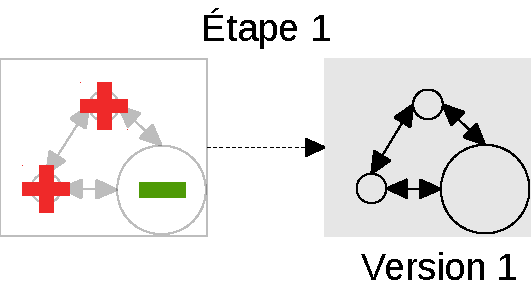
\includegraphics[width = \linewidth, page = 1]{img/schemas_etapes_individuelles.pdf}
	\caption{Étape 1 du paramétrage et résultats.}
\end{figure}

\pagebreak
\subsubsection{Étape 2}
\begin{figure}[H]
	\centering
	\includegraphics[width = \linewidth, page = 2]{img/schemas_etapes_individuelles.pdf}
	\caption{Étape 2 du paramétrage et résultats.}
\end{figure}

\pagebreak
\subsubsection{Étape 3}
\begin{figure}[H]
	\centering
	\includegraphics[width = \linewidth, page = 3]{img/schemas_etapes_individuelles.pdf}
	\caption{Étape 3 du paramétrage et résultats.}
\end{figure}

\pagebreak
\subsubsection{Étape 4}
\begin{figure}[H]
	\centering
	\includegraphics[width = \linewidth, page = 4]{img/schemas_etapes_individuelles.pdf}
	\caption{Étape 4 du paramétrage et résultats.}
\end{figure}

\pagebreak
\subsubsection{Étape 5}
\begin{figure}[H]
	\centering
	\includegraphics[width = \linewidth, page = 5]{img/schemas_etapes_individuelles.pdf}
	\caption{Étape 5 du paramétrage et résultats.}
\end{figure}

\pagebreak
\subsubsection{Étape 6}
\begin{figure}[H]
	\centering
	\includegraphics[width = \linewidth, page = 6]{img/schemas_etapes_individuelles.pdf}
	\caption{Étape 6 du paramétrage et résultats.}
\end{figure}

\pagebreak
\subsubsection{Étape 7}
\begin{figure}[H]
	\centering
	\includegraphics[width = \linewidth, page = 7]{img/schemas_etapes_individuelles.pdf}
	\caption{Étape 7 du paramétrage et résultats.}
\end{figure}

\pagebreak
\subsubsection{Étape 8}
\begin{figure}[H]
	\centering
	\includegraphics[width = \linewidth, page = 8]{img/schemas_etapes_individuelles.pdf}
	\caption{Étape 8 du paramétrage et résultats.}
\end{figure}
	
\pagebreak
\subsection{Un bilan des changements majeurs à l'issu du paramétrage}
	
\begin{figure}[H]
	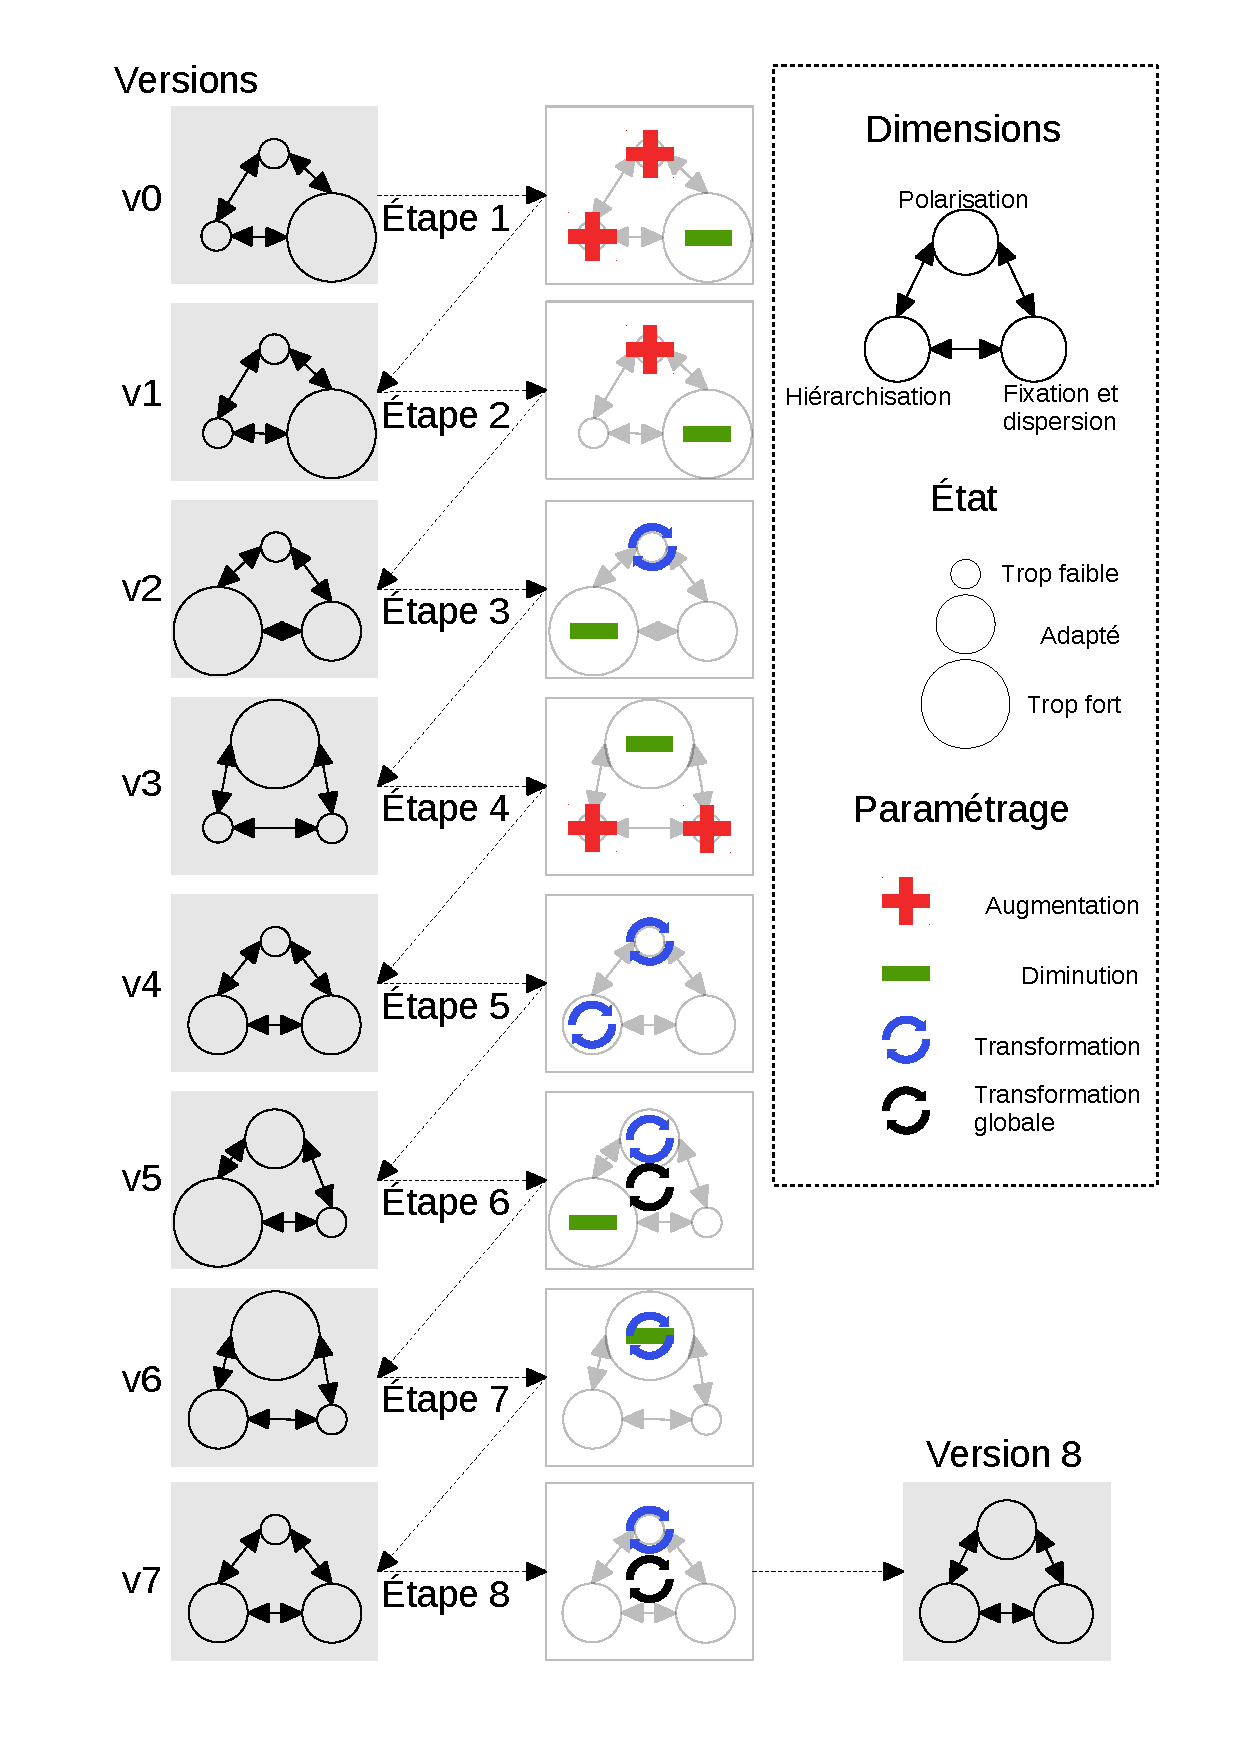
\includegraphics[width = \linewidth, page = 1]{img/schema_etapes_complet.pdf}
	\caption{Schéma récapitulatif et synthétique des étapes du paramétrage de SimFeodal.}
	\label{fig:etapes-parametrage-simfeodal}
\end{figure}
	
	\section{Paramétrage de SimFeodal}
	\subsection{Avant propos sur le paramétrage d'un modèle complexe}
	\subsection{Les étapes du paramètrage de SimFeodal}
	\subsection{Un bilan des changements majeurs à l'issu du paramétrage}
	
	
%		\section{Comment traiter les sorties du modèle ?}
	\subsection{Variabilité}
	- Quelle variabilité du modèle ? Pour quelles raisons (aléa init. vs aléa mécanique) ?
	\subsection{Nombre de sortie}
	- Sorties graphiques, rapports, rapports ++
	\subsection{Masse des sorties}
	- Comment aller plus loin ?
	\section{Comment traiter les sorties du modèle ?}
	\subsection{Variabilité}
	\subsection{Nombre de sortie}
	\subsection{Masse des sorties}

	
%	\printbibliography 
	
\end{document}
